\section{Test of $tbW'$ generation}
\label{sec:PrepareWprime}
Motivation of this section is to check that we can apply same analysis framework to the $tbW'$ search as $tbH^{+}$ search. For that reason, we compared the kinematics of $tbW'$ production with ones of $tbH^{+}$ production in the following sections. As result, there were no significant differences between these productions (Section \ref{subsubsec:ComparisonWpAndHp}). Therefore, we continue to search $tbW'$ production with same analysis framework as $tbH^{+}$ search.

\subsection{$tbW'$ MC generation in private}
\label{subsec:WprimeMCGeneration_InPrivate}
We also search for $W'{\rightarrow}tb$ decay with the seach of $H^{+}{\rightarrow}tb$ decay, where $W'$ is produced in association with $tb$ same as $H^{+}$ production. Before the official MC generation, the private MC samples for both left-handed (LH) and right-handed (RH) $W'$ were generated using MadGraph5\_aMC@NLO. These generated test samples are summarized in Table \ref{tab:WprimeTestSamples}.

\begin{table}[H]
  \centering
  \begin{tabular*}{90mm}{@{\extracolsep{\fill}}c|c|c}
    \hline\hline
    $W'$ mass [GeV] & Type (LH or RH) & Size (events) \\
    \hline
    1000            & LH              & 0.1M\\
    1000            & RH              & 0.1M\\
    \hline
    2000            & LH              & 0.1M\\
    2000            & RH              & 0.1M\\
    \hline
    3000            & LH              & 0.1M\\
    3000            & RH              & 0.1M\\
    \hline
    4000            & LH              & 0.1M\\
    4000            & RH              & 0.1M\\
    \hline
    5000            & LH              & 0.1M\\
    5000            & RH              & 0.1M\\
    \hline\hline
  \end{tabular*}
  \caption{}
  \label{tab:WprimeTestSamples}
\end{table}


\subsection{Kinematics study in truth level}
\label{subsec:WprimeKinematicsStudyInTruthLevel}

\subsubsection{Reconstructed truth objects}
To study the kinematics properties of $W'{\rightarrow}tb$ events in truth level, TruthDAOD samples were produced with \textit{TRUTH1} format \cite{Twiki-TruthDAOD}. The following truth objects are reconstructed according to the official ATLAS truth object definition \cite{ATL-COM-PHYS-2014-439}. Moreover, overlapping objects are removed as shown in Table \ref{tab:TRUTHOLR}. 

\begin{table}[H]
  \centering
  \begin{tabular*}{110mm}{@{\extracolsep{\fill}}cc}
    \hline\hline
    Truth object                           & Collection name\\
    \hline
    Truth electron                         & TruthElectrons\\
    Truth muon                             & TruthMuons\\
    Truth small-R jet ($j^{\text{truth}}$) & AntiKt4TruthDressedWZJets\\
    Truth large-R jet ($J^{\text{truth}}$) & AntiKt10TruthTrimmedPtFrac5SmallR20Jets\\
    \hline\hline
  \end{tabular*}
  \caption{List of reconstructed truth objects in this study. Each object is selected from the indicated collection of with their corresponding aux containers.}
  \label{tab:TruthObjects}
\end{table}

\begin{table}[H]
  \centering
  \begin{tabular*}{100mm}{lll}
    \hline\hline
    \multicolumn{1}{c}{Reject} & \multicolumn{1}{c}{Against}  & \multicolumn{1}{c}{Criteria}\\
    \hline
    Truth large-$R$ jet        & Truth electron               & ${\Delta}R<1.0$\\
    Truth small-$R$ jet        & Truth large-R jet            & ${\Delta}R<1.0$\\
    \hline\hline
  \end{tabular*}
  \caption{Summary of overlap removal procedures among truth objects}
  \label{tab:TRUTHOLR}
\end{table}


\subsubsection{Event selection}
To study in the same phase space as the "SR" in Section \ref{subsec:EventSelection_SR}, events are selected according to the number of truth leptons, small-R jets and large-R jets as shown in Table \ref{tab:TruthEventSelection}.

\begin{table}[H]
  \centering
  \begin{tabular*}{150mm}{lll}
    \hline\hline
    \multicolumn{1}{c}{Cut}                               & \multicolumn{2}{c}{Criteria}\\
    \hline
    Truth leptons                                         & \multicolumn{2}{c}{\textbf{Exactly 1 truth lepton in event}}\\
    \multicolumn{1}{c}{(${\ell}^{\text{truth}}$)}         & \underline{Truth electron}          & \underline{Truth muon}\\
                                                          & $p_{\text{T}}>27$ GeV               & $p_{\text{T}}>27$ GeV\\
                                                          & $|\eta|<1.37$ or $1.52<|\eta|<2.47$ & $|\eta|<2.5$\\
    \hline
    Truth large-$R$ jets                                  & \multicolumn{2}{c}{\textbf{${\geq}1$ truth large-$R$ jets}}\\
    originated from top-quark                             & \multicolumn{2}{l}{$350\text{GeV}<p_{\text{T}}<2500\text{GeV}$}\\
    \multicolumn{1}{c}{($J_{\text{top}}^{\text{truth}}$)} & \multicolumn{2}{l}{$|\eta|<2.0$}\\
                                                          & \multicolumn{2}{l}{${\Delta}R(t, J_{\text{top}}^{\text{truth}})<1.0$ or ${\Delta}R(\bar{t}, J_{\text{top}}^{\text{truth}})<1.0$}\\
                                                          & \multicolumn{2}{l}{($t (\bar{t})$: truth particle labelled as PDG ID=6 (-6))}\\
    \hline
    Truth small-$R$ jets                                  & \multicolumn{2}{c}{\textbf{${\geq}2$ truth small-$R$ jets}}\\
    originated from $b$-quark                             & \multicolumn{2}{l}{$p_{\text{T}}>25$ GeV}\\
    \multicolumn{1}{c}{($b$-jet$^{\text{truth}}$)}        & \multicolumn{2}{l}{$|\eta|<2.5$}\\
                                                          & \multicolumn{2}{l}{PDG ID of the highest-E ghost parton is 5}\\
    \hline\hline
  \end{tabular*}
  \caption{Summary of event selections in truth level.}
  \label{tab:TruthEventSelection}
\end{table}


\subsubsection{Kinematics comparison with $tbH^{+}$ events}
\label{subsubsec:ComparisonWpAndHp}

Variables input to BDT training in Section \ref{subsubsec:BDTInputVars} were defined in truth level as shown in Table \ref{tab:BDTInputVariablesInTruthLevel}. These distributions are compared between $tbW'$ and $tbH^{+}$ in Figure \ref{fig:HpOVERWp_TruthLevel_1000GeV} to \ref{fig:HpOVERWp_TruthLevel_5000GeV}. These were no significant differences.

\begin{table}[H]
  \centering
  \begin{tabular*}{150mm}{@{\extracolsep{\fill}}ll}
    \hline
    \multicolumn{1}{c}{Symbol} & \multicolumn{1}{c}{Description}\\
    \hline\hline
    Truth\_HT\_jets            & Scalar sum of the transverse energy of leading $J_{\text{top}}^{\text{truth}}$ and all $j^{\text{truth}}$\\
    Truth\_LeadingJet\_pt      & Leading $j^{\text{truth}}$ $p_\text{T}$\\
    Truth\_Mjjj\_MaxPt         & Invariant mass of the $j^{\text{truth}}$ triplet with maximum $p_\text{T}$\\
    Truth\_Mbb\_MaxPt          & Invariant mass of the $b$-jet$^{\text{truth}}$ pair with maximum $p_\text{T}$\\
    Truth\_Muu\_MindR          & Invariant mass of the $j^{\text{truth}}$-pair with minimum $\Delta{R}$ except for $b$-jet$^{\text{truth}}$\\
    Truth\_dRlepbb\_MindR      & $\Delta{R}$ between ${\ell}^{\text{truth}}$ and the pair of $b$-jet$^{\text{truth}}$ with smallest $\Delta{R}$\\
    Truth\_dRbb\_avg           & Average $\Delta{R}$ between all $b$-jet$^{\text{truth}}$ pairs in the event\\
    Truth\_Centrality\_all     & Centrality calculated using leading $J_{\text{top}}^{\text{truth}}$, all $j^{\text{truth}}$ and ${\ell}^{\text{truth}}$\\
    Truth\_H1\_all             & Second Fox-Wolfram moment calculated using all $j^{\text{truth}}$ and ${\ell}^{\text{truth}}$\\
    Truth\_LeadingTop\_pt      & Leading $J_{\text{top}}^{\text{truth}}$ $p_\text{T}$\\
    Truth\_LeadingTop\_m       & Invariant mass of leading $J_{\text{top}}^{\text{truth}}$ \\
    Truth\_Pt\_tb              & $p_\text{T}$ of the pair of leading $J_{\text{top}}^{\text{truth}}$ and leading $b$-jet$^{\text{truth}}$\\
    Truth\_M\_tb               & Invariant mass of the pair of leading $J_{\text{top}}^{\text{truth}}$ and leading $b$-jet$^{\text{truth}}$\\
    Truth\_PtAsymm\_tb         & $p_\text{T}$ asymmetry between leading $J_{\text{top}}^{\text{truth}}$ and leading $b$-jet$^{\text{truth}}$\\
    \hline
  \end{tabular*}
  \caption{Definition of variables input to BDT training in truth level.}
  \label{tab:BDTInputVariablesInTruthLevel}
\end{table}


\begin{figure}[H]
  \subfloat[Truth\_HT\_jets] {
    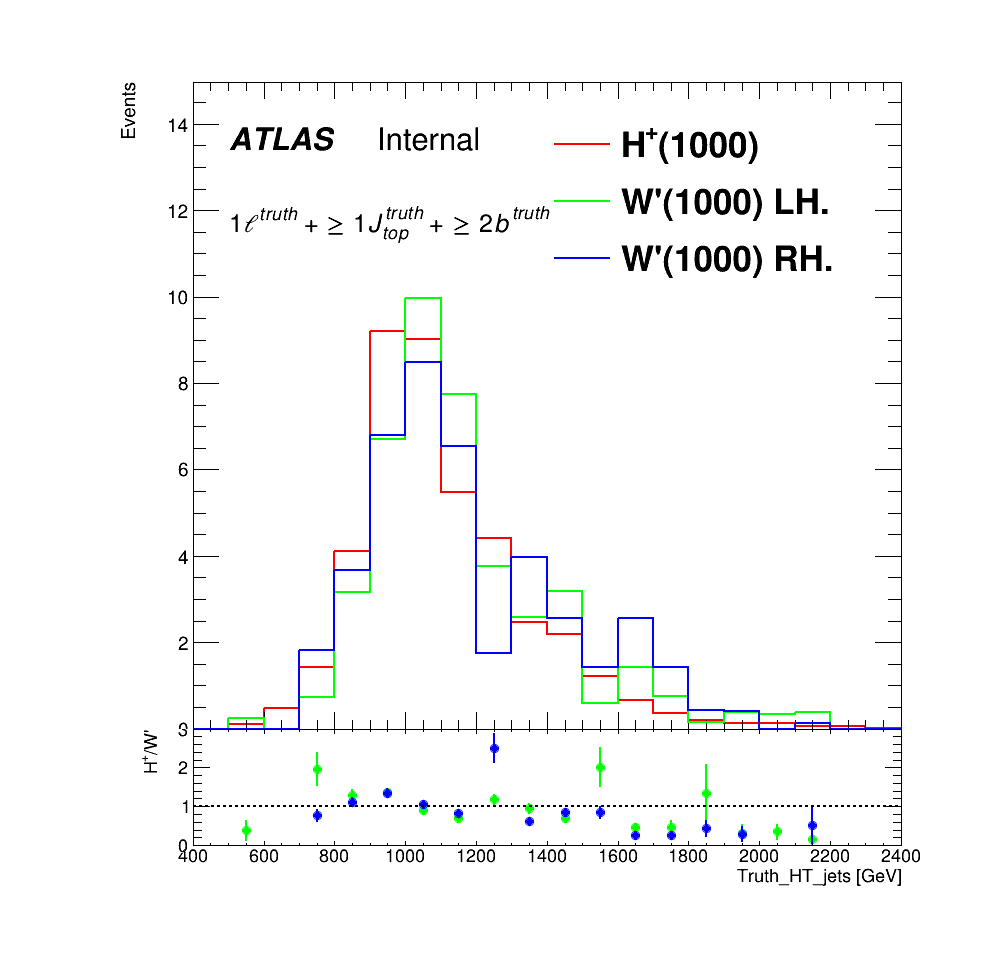
\includegraphics[width=0.25\textwidth]{images/WpMCTest/Comparison_HT_jets_1000GeV.png}
    \label{fig:HpOVERWp_HT_jets_1000GeV}
  }
  \subfloat[Truth\_LeadingJet\_pt] {
    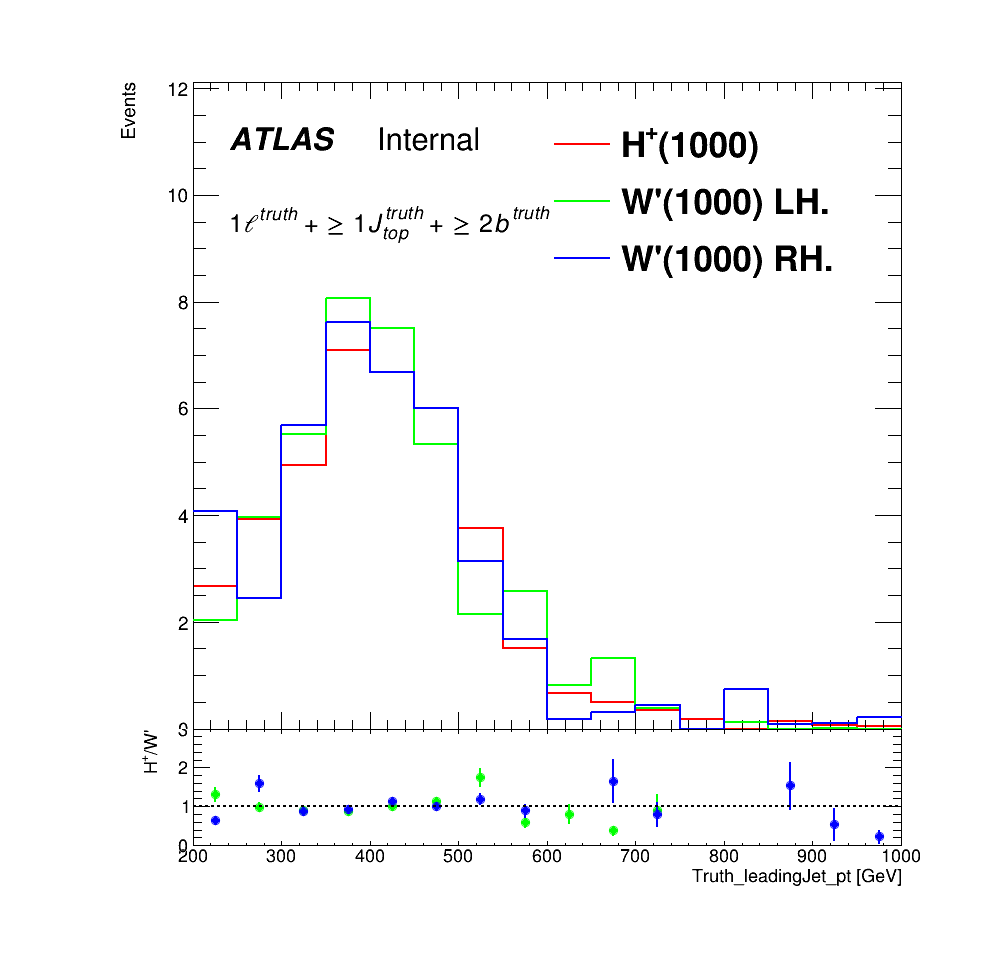
\includegraphics[width=0.25\textwidth]{images/WpMCTest/Comparison_leadingJet_pt_1000GeV.png}
    \label{fig:HpOVERWp_LeadingJet_pt_1000GeV}
  }
  \subfloat[Truth\_Centrality\_all] {
    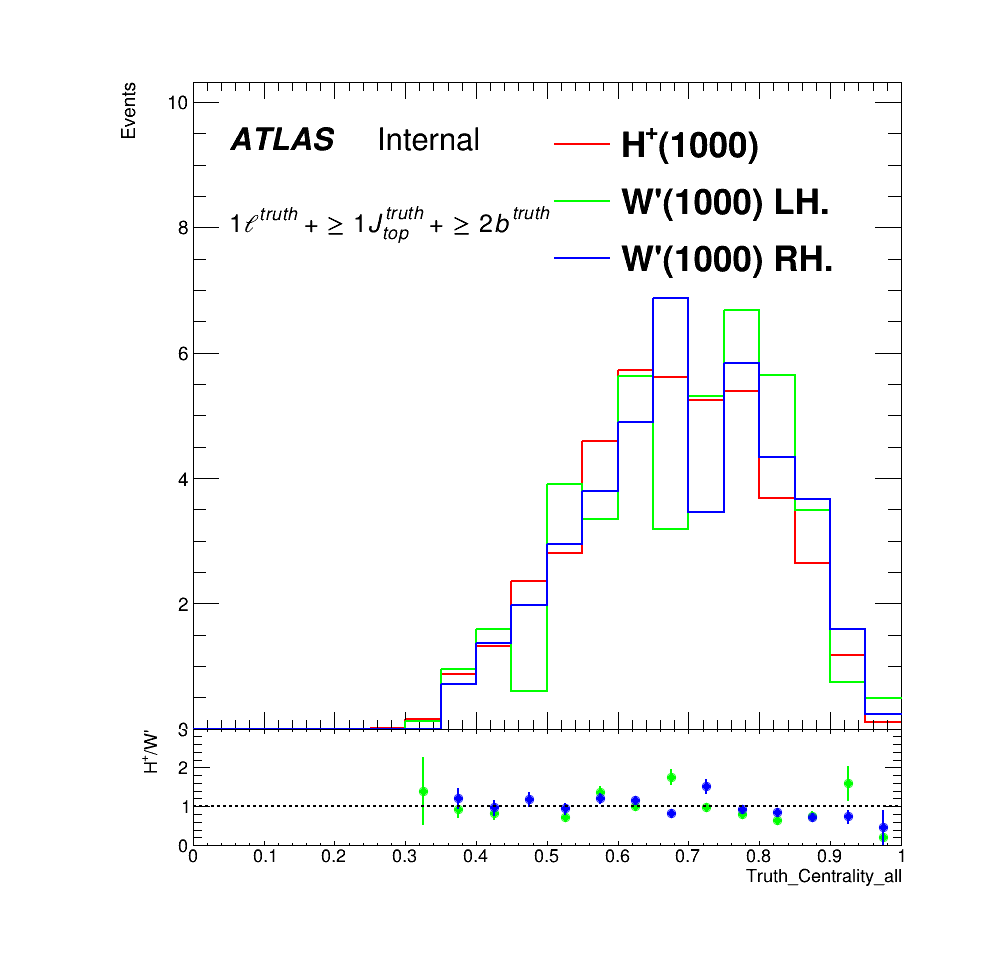
\includegraphics[width=0.25\textwidth]{images/WpMCTest/Comparison_Centrality_all_1000GeV.png}
    \label{fig:HpOVERWp_Centrality_all_1000GeV}
  }
  \subfloat[Truth\_H1\_all] {
    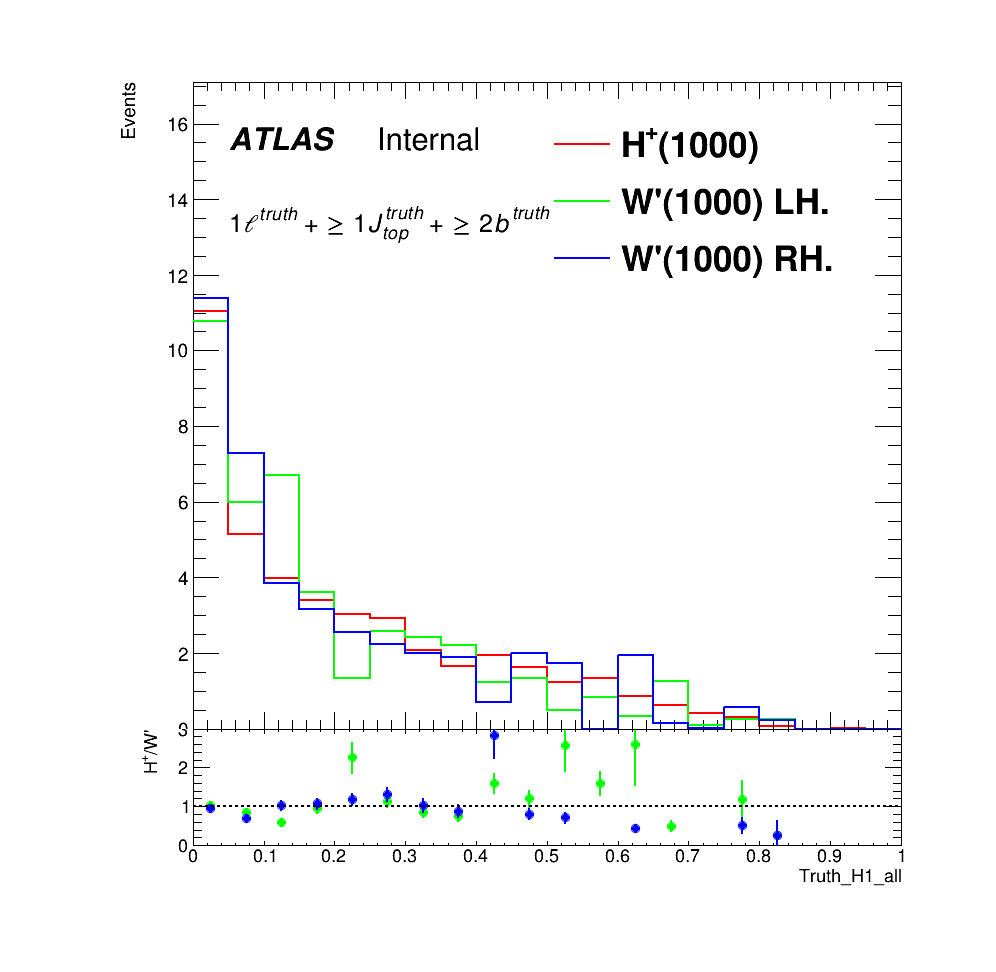
\includegraphics[width=0.25\textwidth]{images/WpMCTest/Comparison_H1_all_1000GeV.png}
    \label{fig:HpOVERWp_H1_all_1000GeV}
  }\\
  \subfloat[Truth\_Mbb\_MaxPt] {
    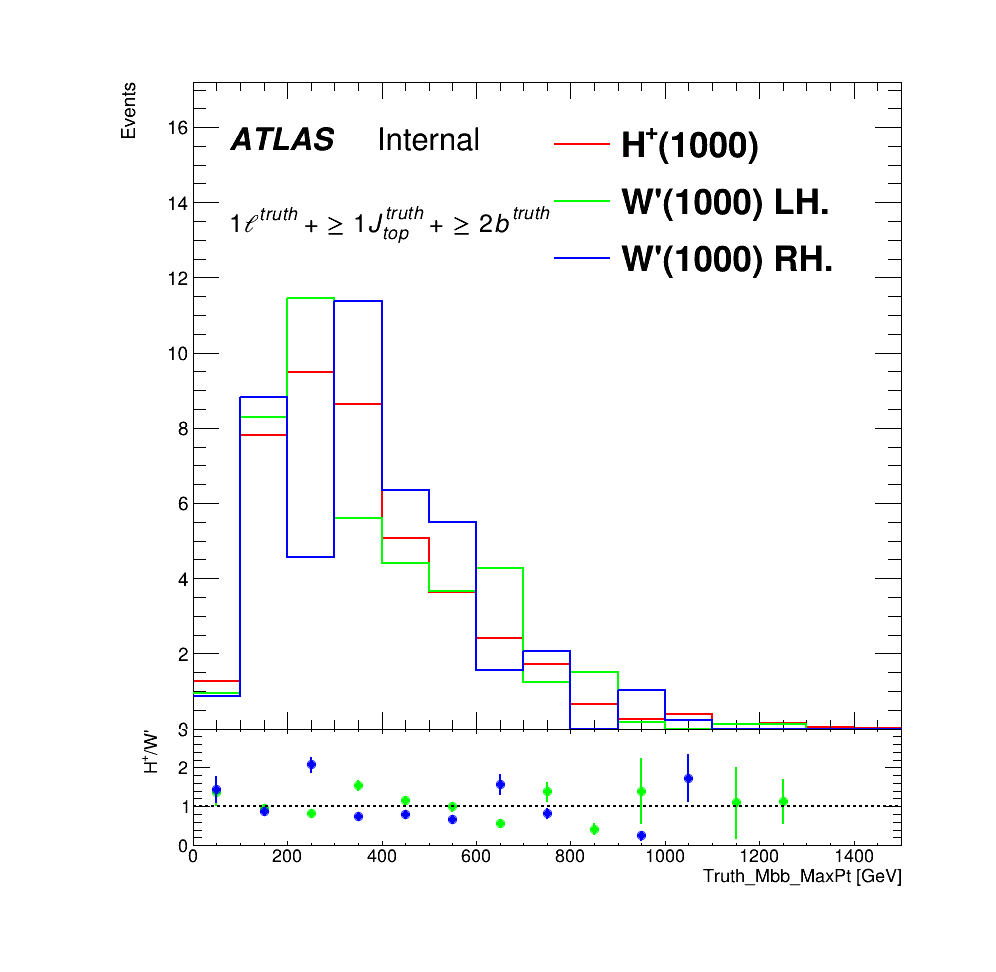
\includegraphics[width=0.25\textwidth]{images/WpMCTest/Comparison_Mbb_MaxPt_1000GeV.png}
    \label{fig:HpOVERWp_Mbb_MaxPt_1000GeV}
  }
  \subfloat[Truth\_Mjjj\_MaxPt] {
    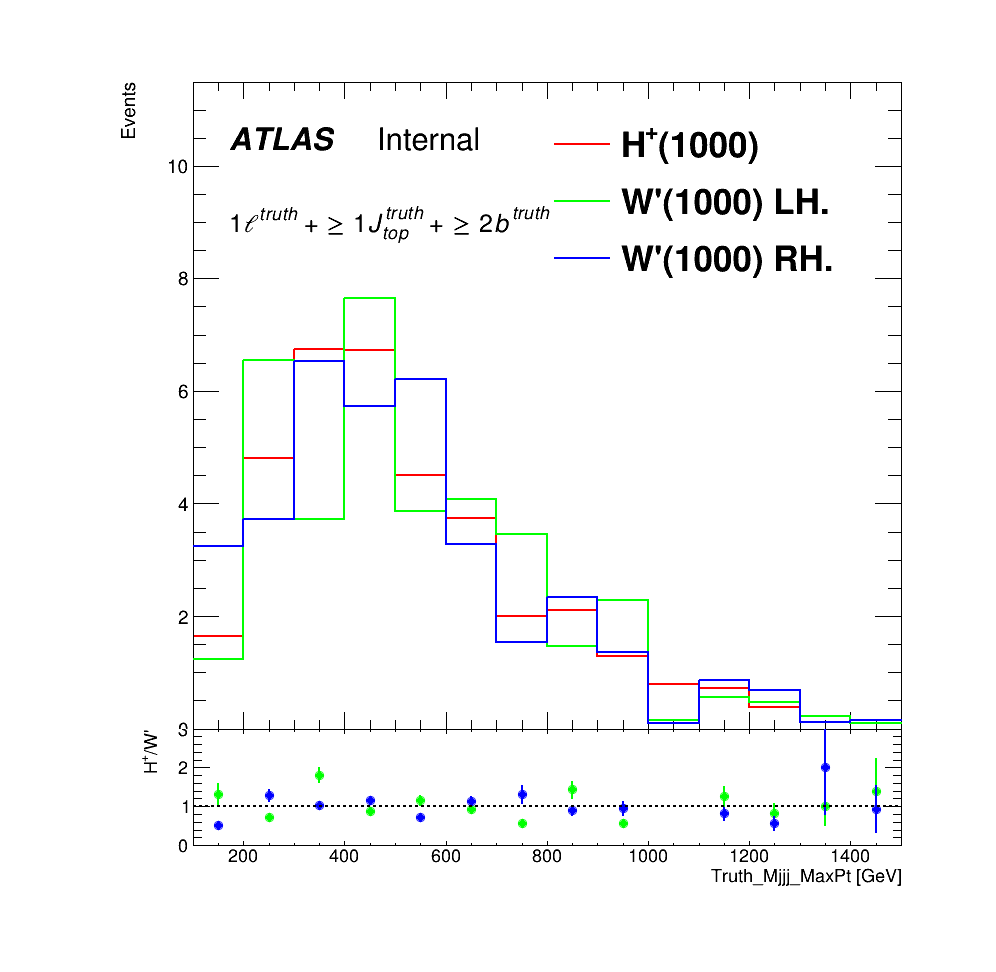
\includegraphics[width=0.25\textwidth]{images/WpMCTest/Comparison_Mjjj_MaxPt_1000GeV.png}
    \label{fig:HpOVERWp_Mjjj_MaxPt_1000GeV}
  }
  \subfloat[Truth\_Muu\_MindR] {
    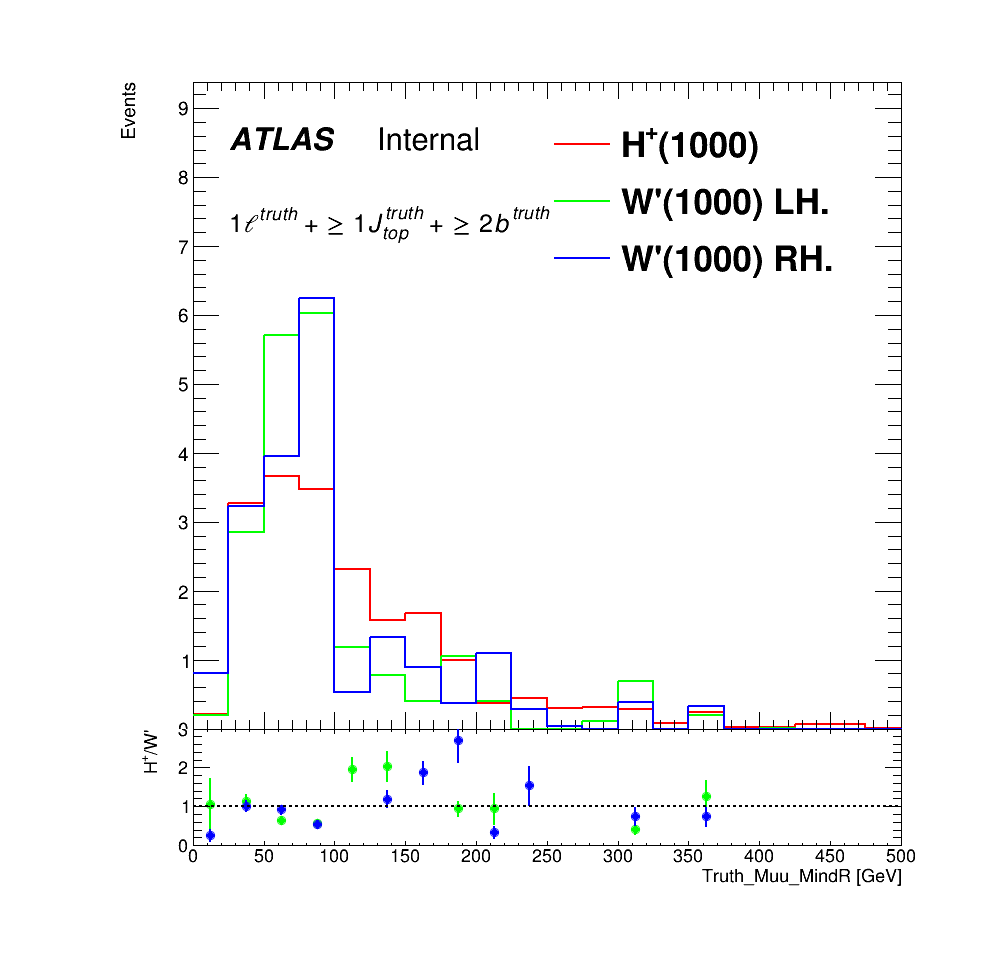
\includegraphics[width=0.25\textwidth]{images/WpMCTest/Comparison_Muu_MindR_1000GeV.png}
    \label{fig:HpOVERWp_Muu_MindR_1000GeV}
  }
  \subfloat[Truth\_dRbb\_avg] {
    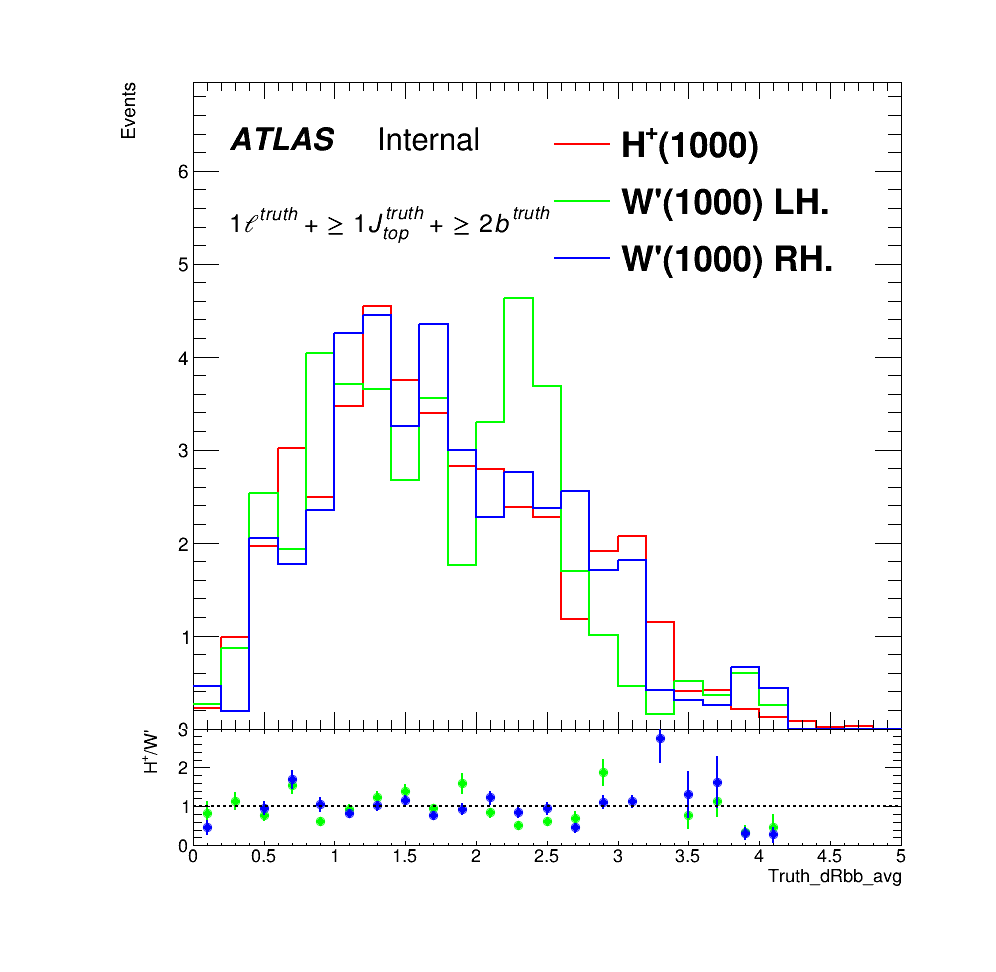
\includegraphics[width=0.25\textwidth]{images/WpMCTest/Comparison_dRbb_avg_1000GeV.png}
    \label{fig:HpOVERWp_dRbb_avg_1000GeV}
  }\\
  \subfloat[Truth\_dRlepbb\_MindR] {
    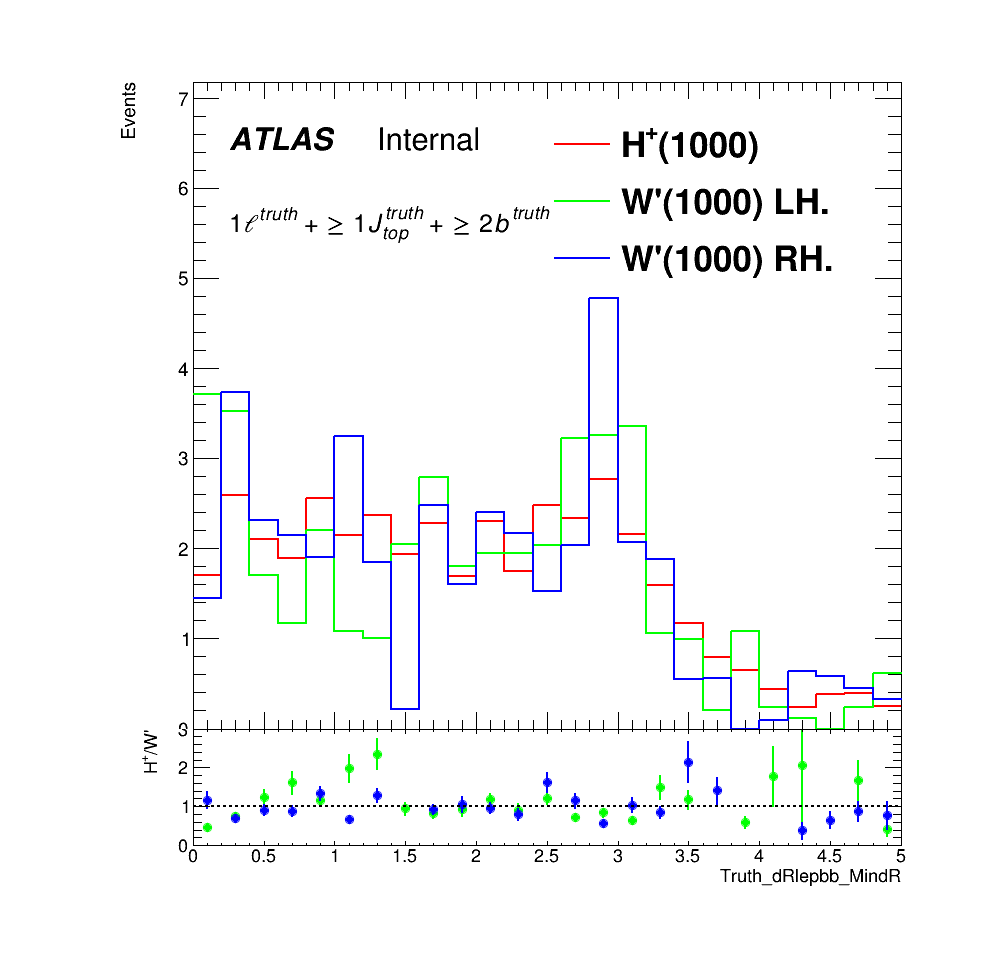
\includegraphics[width=0.25\textwidth]{images/WpMCTest/Comparison_dRlepbb_MindR_1000GeV.png}
    \label{fig:HpOVERWp_dRlepbb_MindR_1000GeV}
  }
  \subfloat[Truth\_LeadingTop\_m] {
    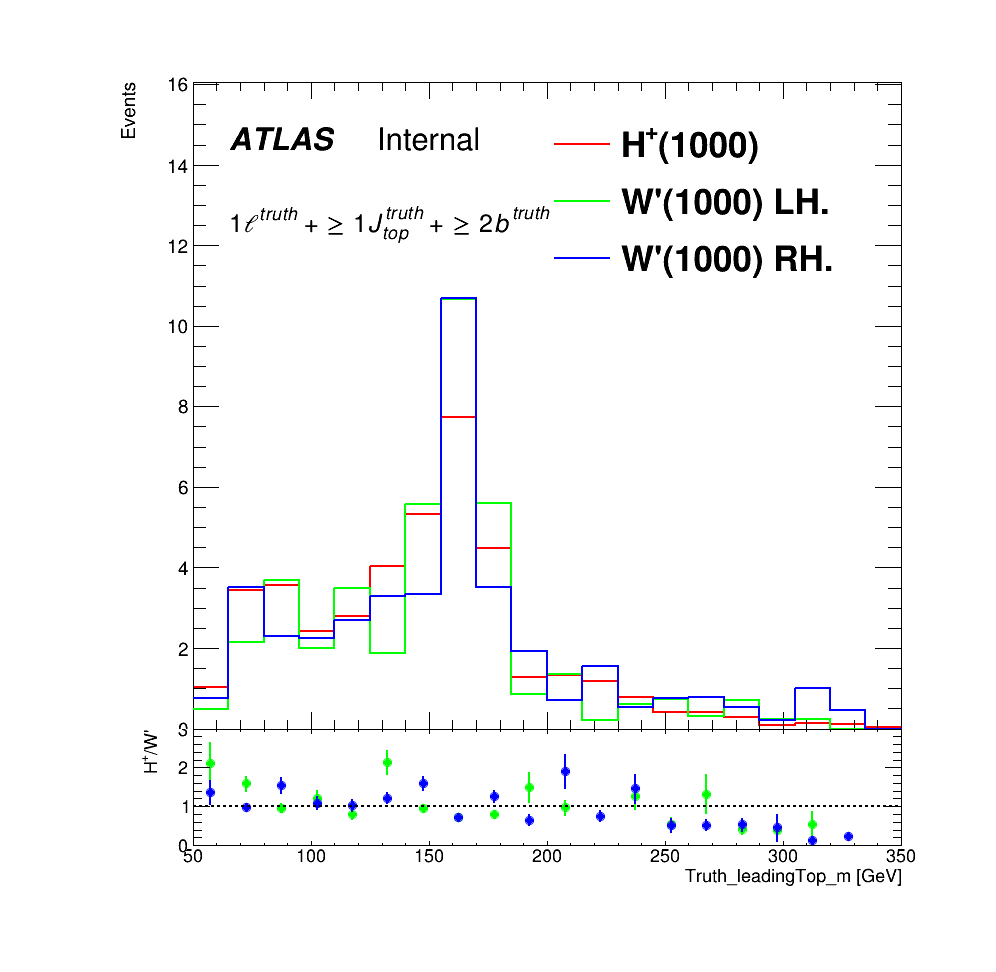
\includegraphics[width=0.25\textwidth]{images/WpMCTest/Comparison_leadingTop_m_1000GeV.png}
    \label{fig:HpOVERWp_LeadingTop_mass_1000GeV}
  }
  \subfloat[Truth\_LeadingTop\_pt] {
    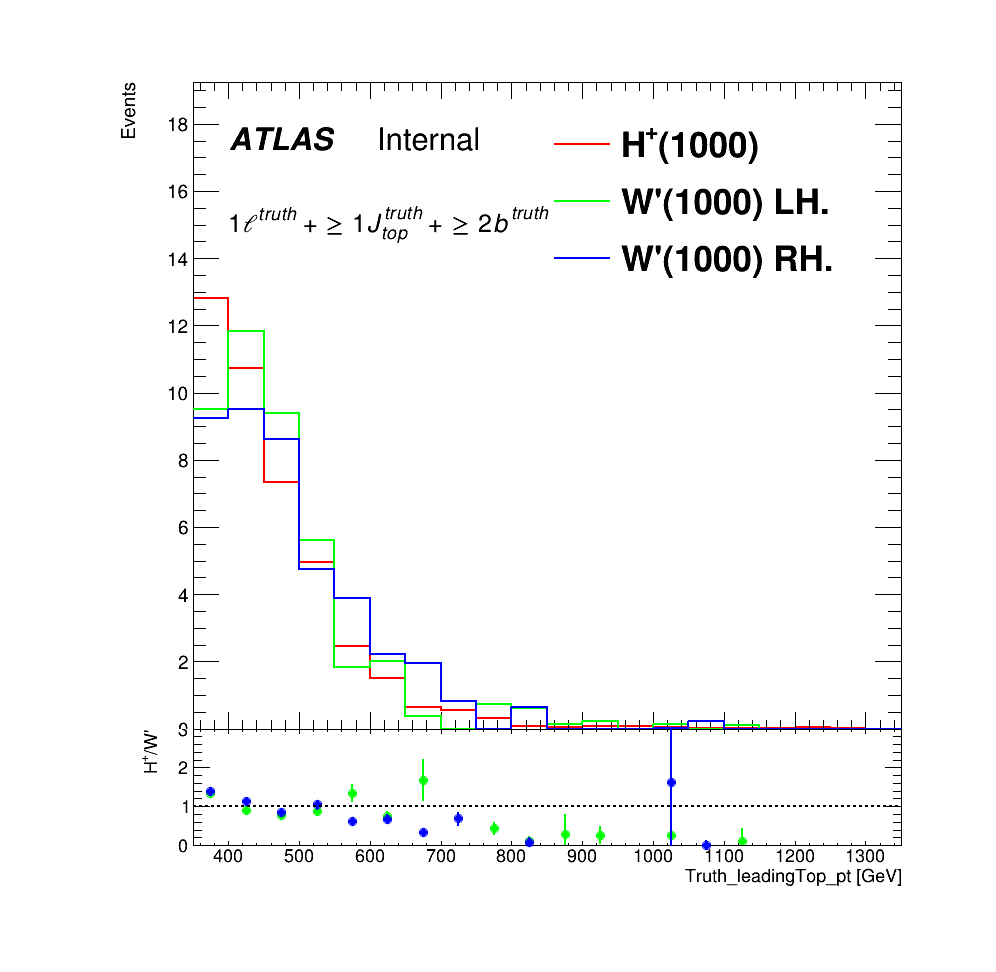
\includegraphics[width=0.25\textwidth]{images/WpMCTest/Comparison_leadingTop_pt_1000GeV.png}
    \label{fig:HpOVERWp_LeadingTop_pt_1000GeV}
  }
  \subfloat[Truth\_M\_tb] {
    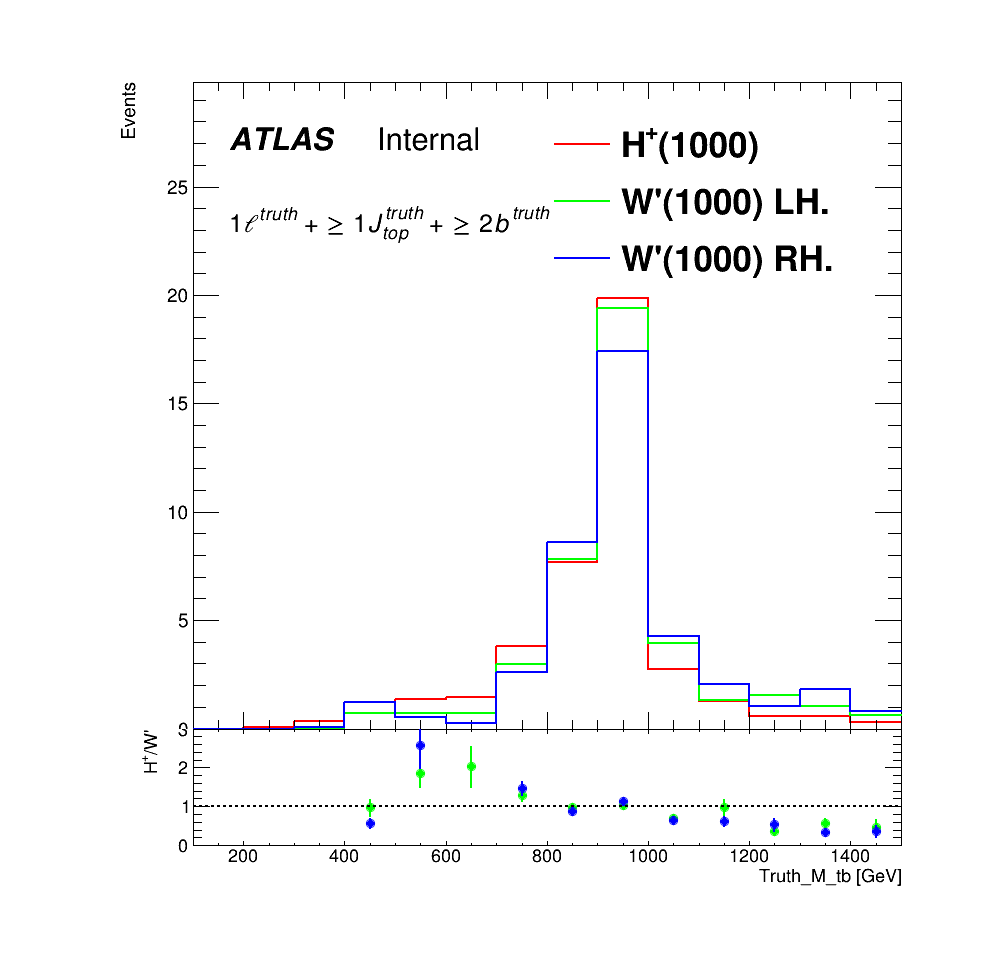
\includegraphics[width=0.25\textwidth]{images/WpMCTest/Comparison_tb_m_1000GeV.png}
    \label{fig:HpOVERWp_tb_mass_1000GeV}
  }\\
  \subfloat[Truth\_Pt\_tb] {
    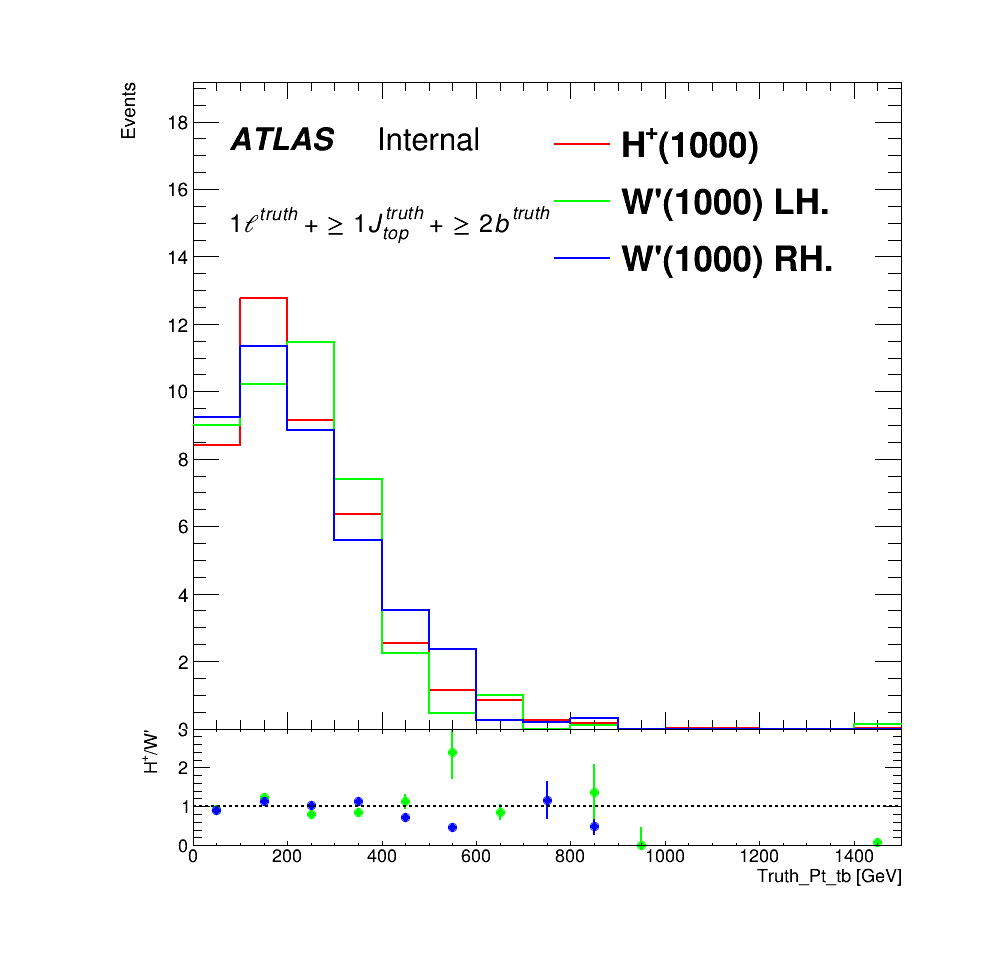
\includegraphics[width=0.25\textwidth]{images/WpMCTest/Comparison_tb_pt_1000GeV.png}
    \label{fig:HpOVERWp_tb_pt_1000GeV}
  }
  \subfloat[Truth\_PtAsymm\_tb] {
    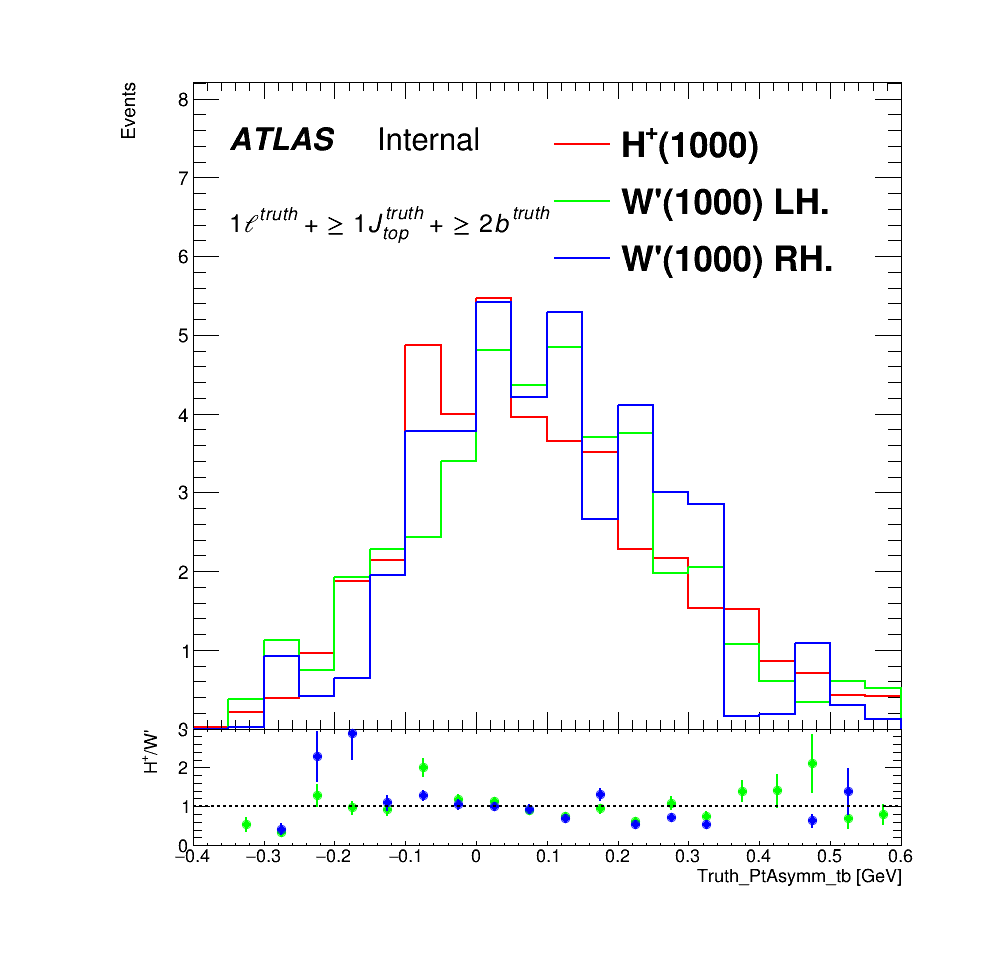
\includegraphics[width=0.25\textwidth]{images/WpMCTest/Comparison_tb_ptAsymm_1000GeV.png}
    \label{fig:HpOVERWp_tb_ptAsymm_1000GeV}
  }
  \caption{Comparison of the kinematic variables between $tbW'$ and $tbH^{+}$ in truth level on 1000 GeV mass hypothesis.}
  \label{fig:HpOVERWp_TruthLevel_1000GeV}
\end{figure}


\begin{figure}[H]
  \subfloat[Truth\_HT\_jets] {
    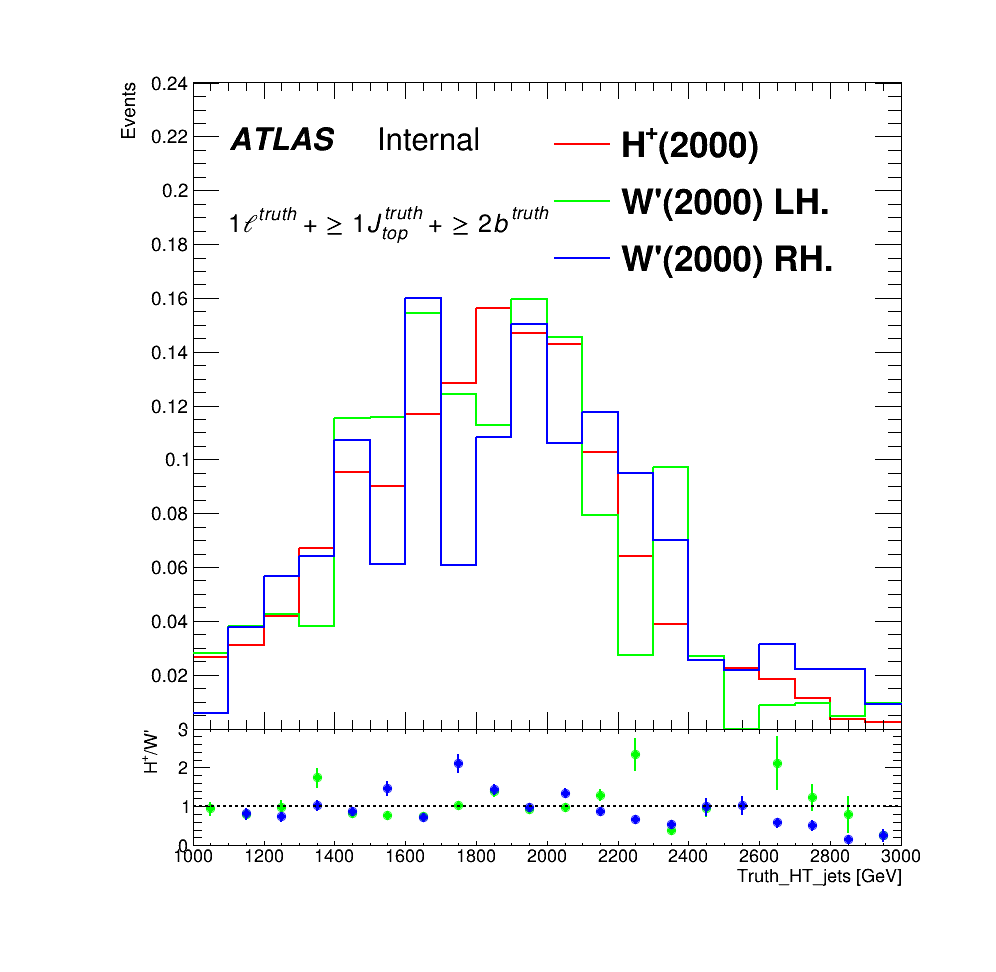
\includegraphics[width=0.25\textwidth]{images/WpMCTest/Comparison_HT_jets_2000GeV.png}
    \label{fig:HpOVERWp_HT_jets_2000GeV}
  }
  \subfloat[Truth\_LeadingJet\_pt] {
    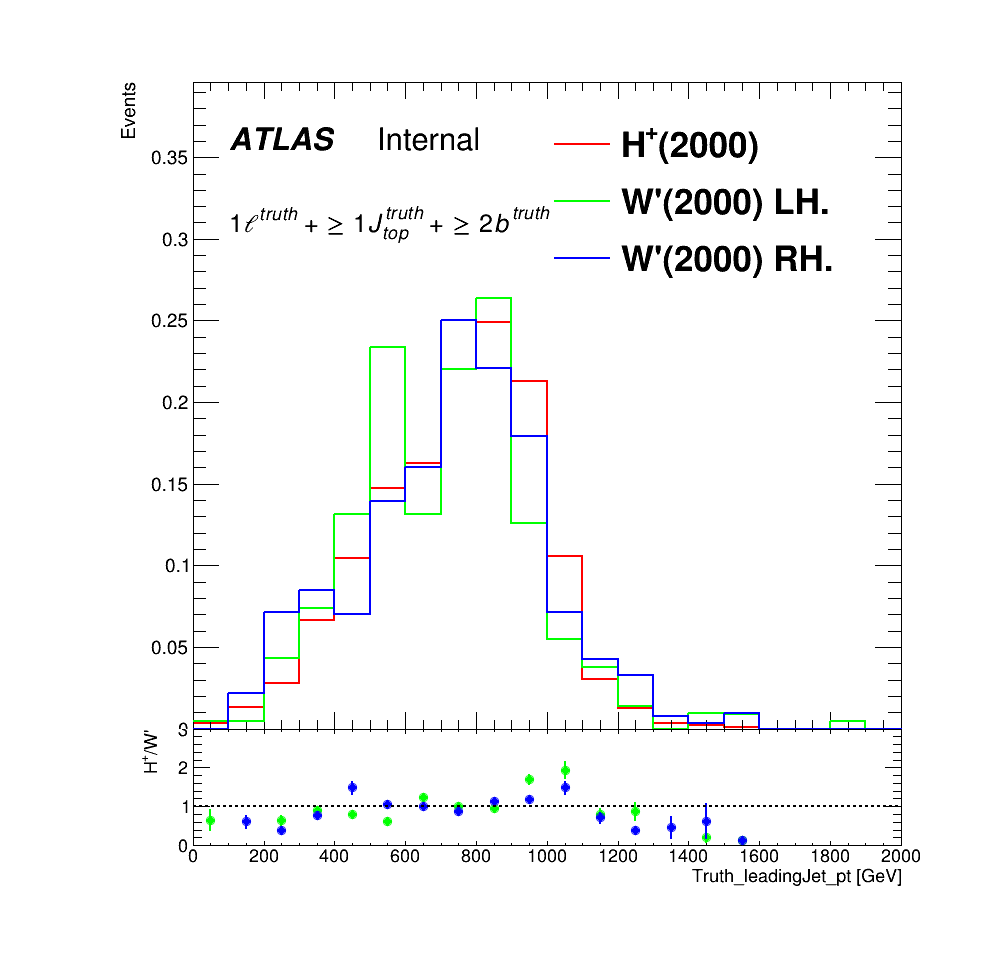
\includegraphics[width=0.25\textwidth]{images/WpMCTest/Comparison_leadingJet_pt_2000GeV.png}
    \label{fig:HpOVERWp_LeadingJet_pt_2000GeV}
  }
  \subfloat[Truth\_Centrality\_all] {
    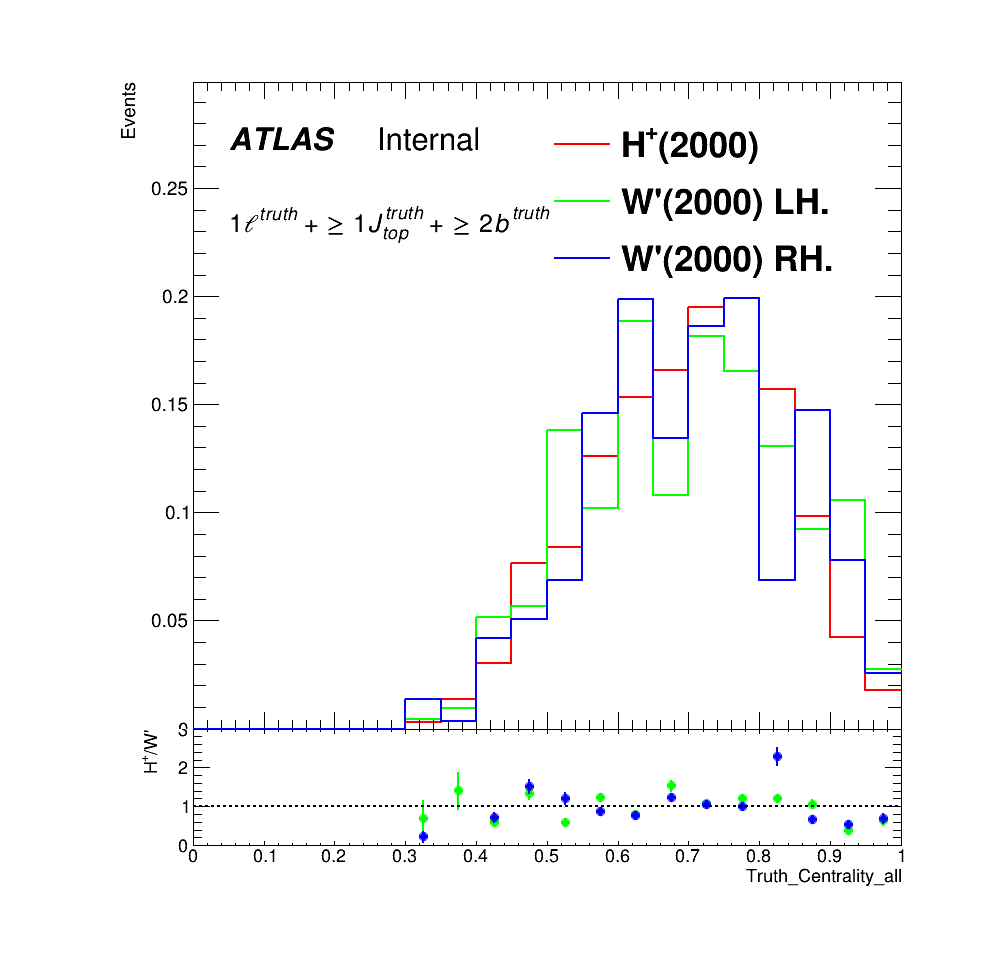
\includegraphics[width=0.25\textwidth]{images/WpMCTest/Comparison_Centrality_all_2000GeV.png}
    \label{fig:HpOVERWp_Centrality_all_2000GeV}
  }
  \subfloat[Truth\_H1\_all] {
    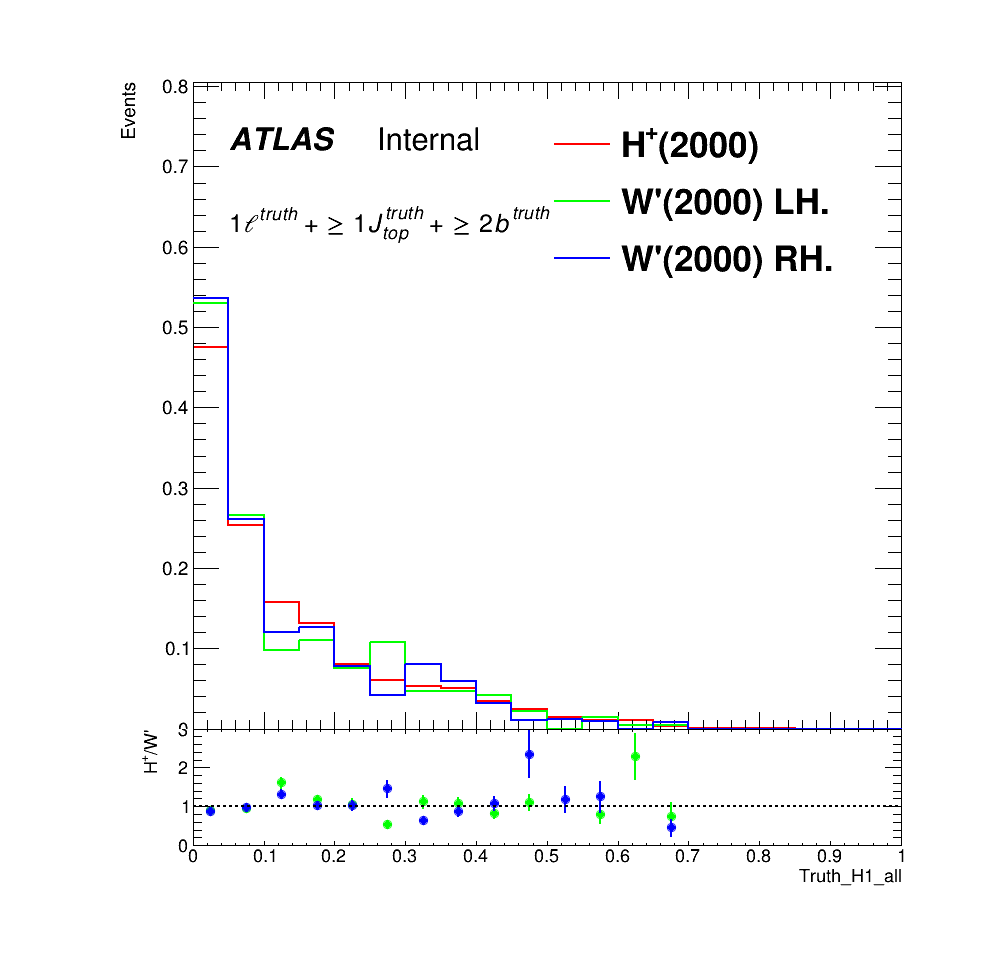
\includegraphics[width=0.25\textwidth]{images/WpMCTest/Comparison_H1_all_2000GeV.png}
    \label{fig:HpOVERWp_H1_all_2000GeV}
  }\\
  \subfloat[Truth\_Mbb\_MaxPt] {
    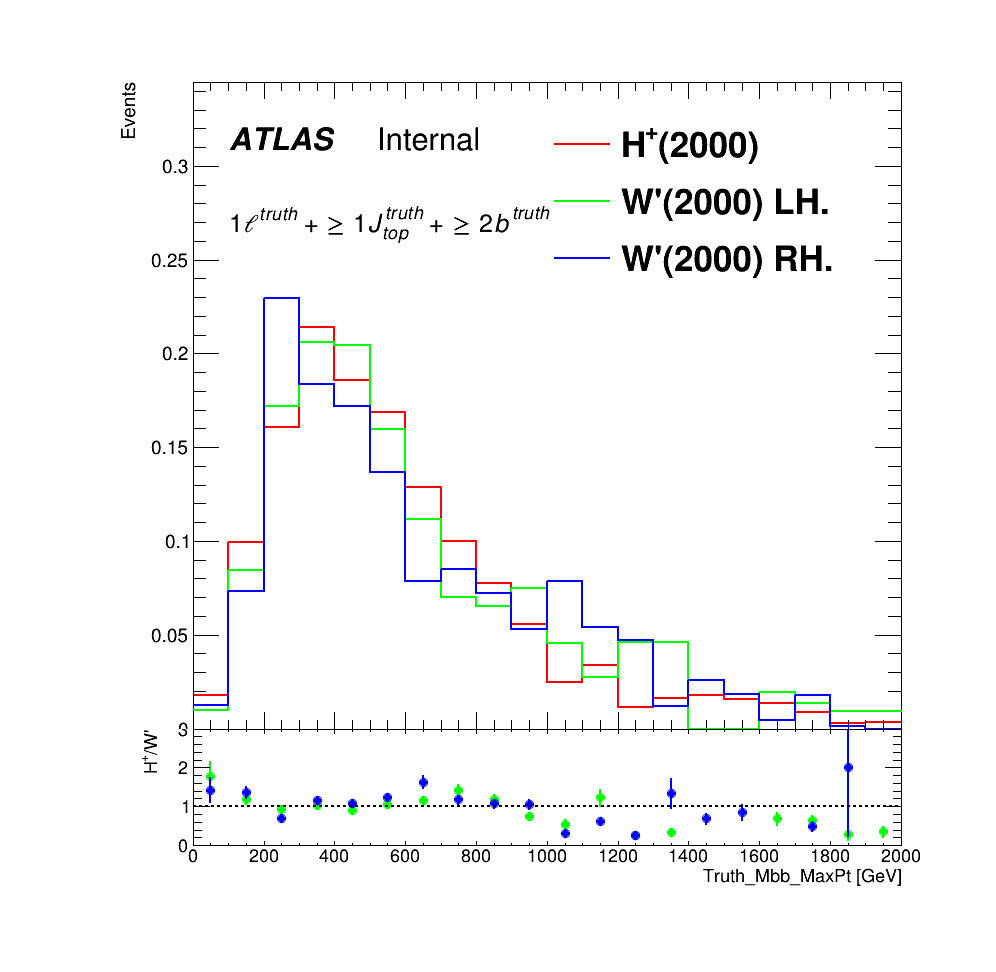
\includegraphics[width=0.25\textwidth]{images/WpMCTest/Comparison_Mbb_MaxPt_2000GeV.png}
    \label{fig:HpOVERWp_Mbb_MaxPt_2000GeV}
  }
  \subfloat[Truth\_Mjjj\_MaxPt] {
    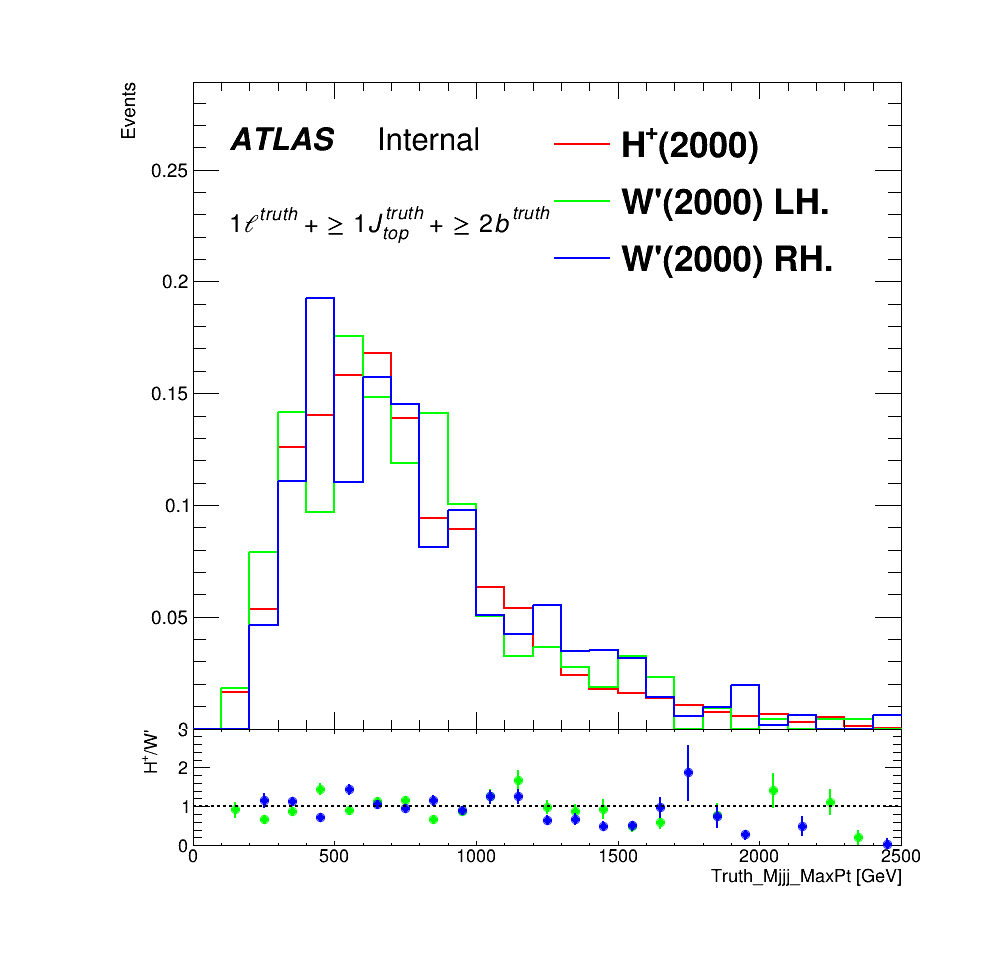
\includegraphics[width=0.25\textwidth]{images/WpMCTest/Comparison_Mjjj_MaxPt_2000GeV.png}
    \label{fig:HpOVERWp_Mjjj_MaxPt_2000GeV}
  }
  \subfloat[Truth\_Muu\_MindR] {
    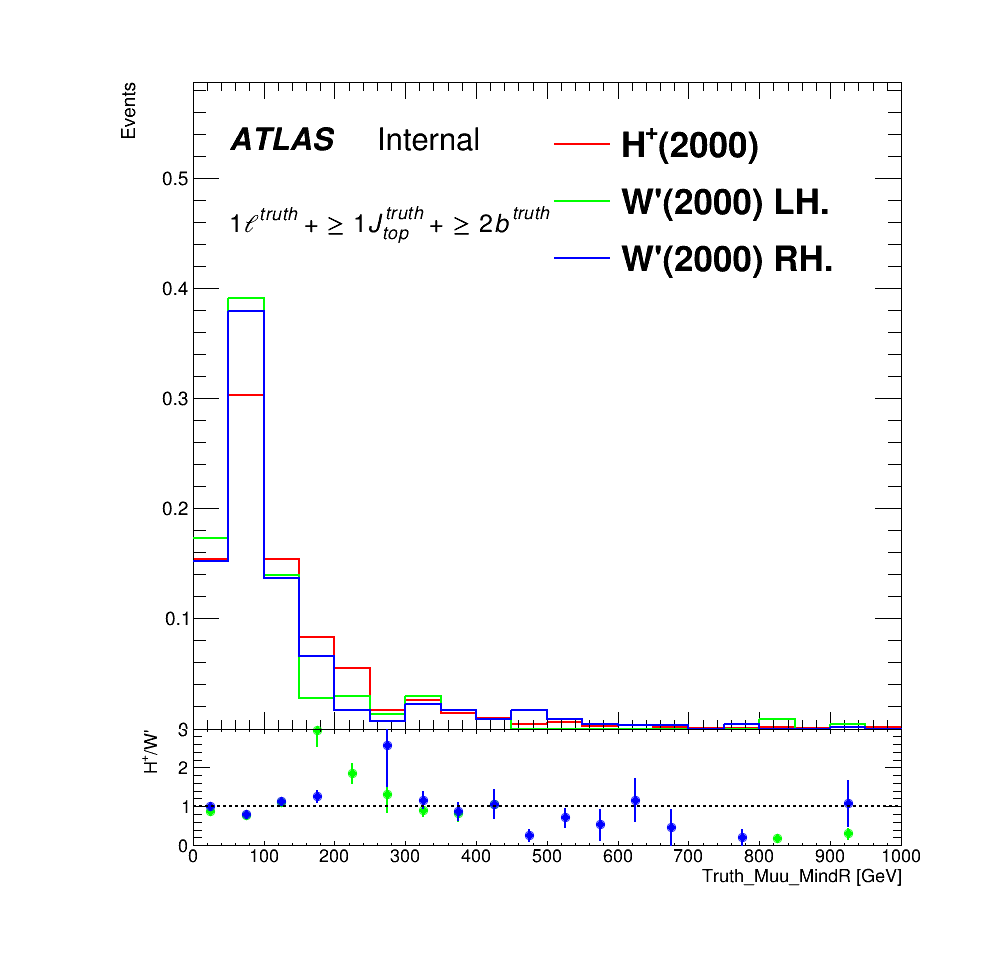
\includegraphics[width=0.25\textwidth]{images/WpMCTest/Comparison_Muu_MindR_2000GeV.png}
    \label{fig:HpOVERWp_Muu_MindR_2000GeV}
  }
  \subfloat[Truth\_dRbb\_avg] {
    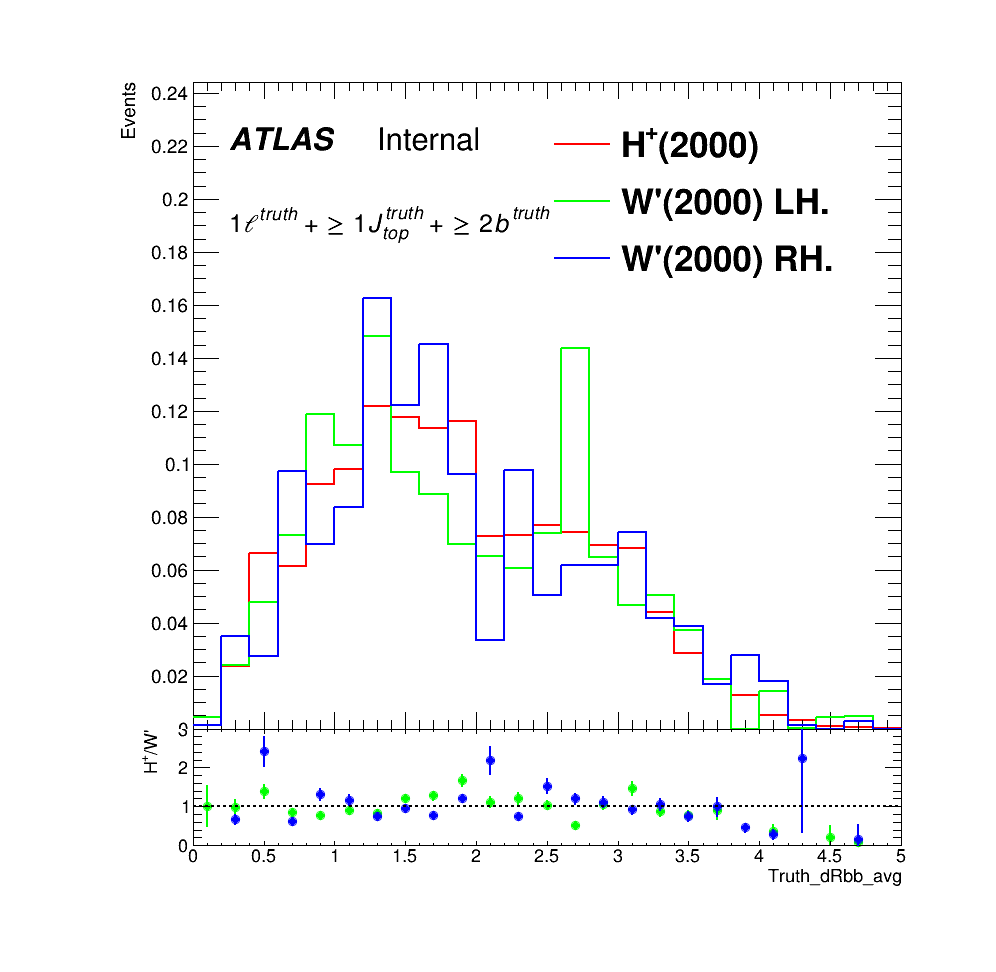
\includegraphics[width=0.25\textwidth]{images/WpMCTest/Comparison_dRbb_avg_2000GeV.png}
    \label{fig:HpOVERWp_dRbb_avg_2000GeV}
  }\\
  \subfloat[Truth\_dRlepbb\_MindR] {
    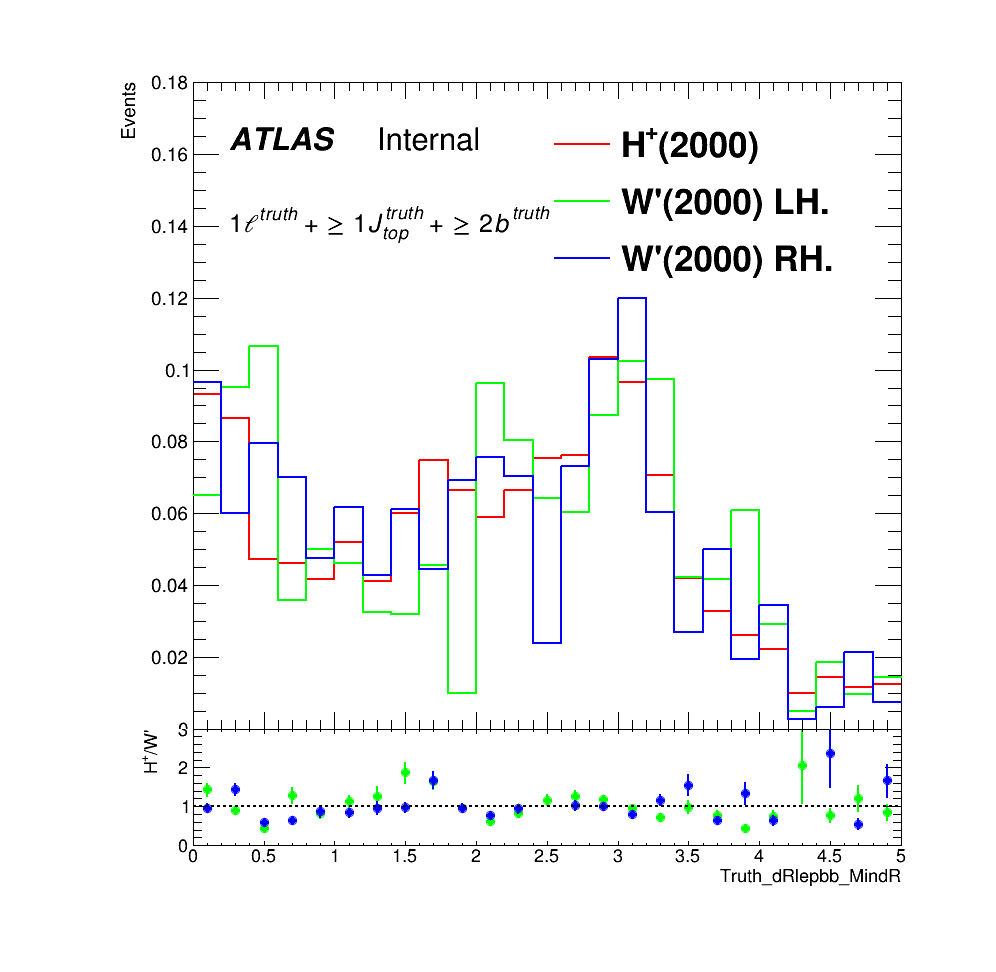
\includegraphics[width=0.25\textwidth]{images/WpMCTest/Comparison_dRlepbb_MindR_2000GeV.png}
    \label{fig:HpOVERWp_dRlepbb_MindR_2000GeV}
  }
  \subfloat[Truth\_LeadingTop\_m] {
    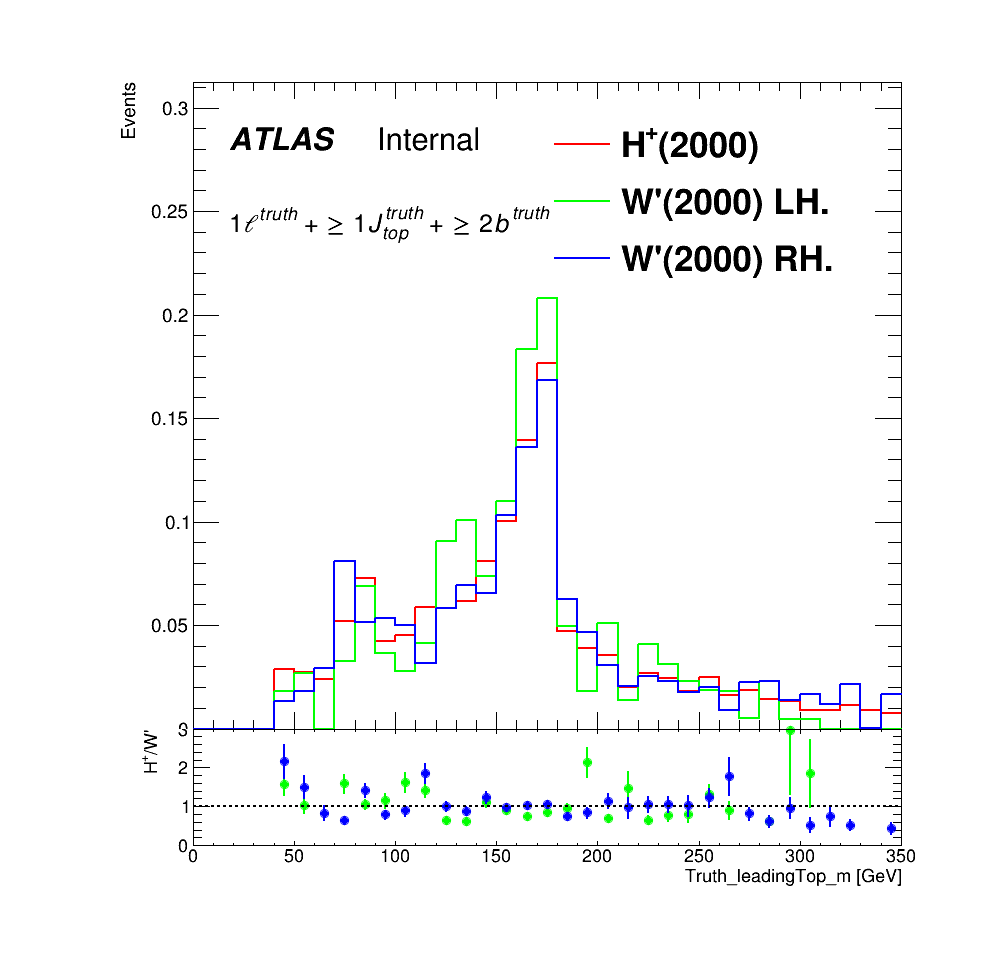
\includegraphics[width=0.25\textwidth]{images/WpMCTest/Comparison_leadingTop_m_2000GeV.png}
    \label{fig:HpOVERWp_LeadingTop_mass_2000GeV}
  }
  \subfloat[Truth\_LeadingTop\_pt] {
    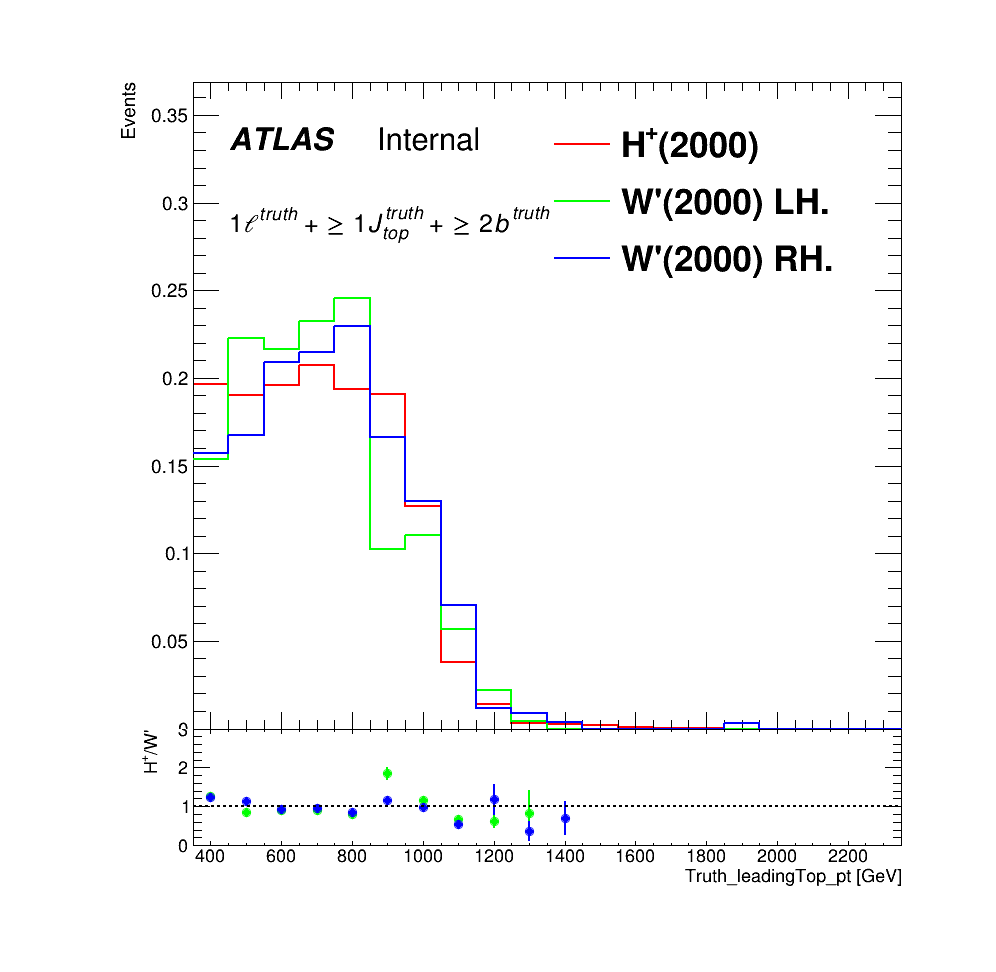
\includegraphics[width=0.25\textwidth]{images/WpMCTest/Comparison_leadingTop_pt_2000GeV.png}
    \label{fig:HpOVERWp_LeadingTop_pt_2000GeV}
  }
  \subfloat[Truth\_M\_tb] {
    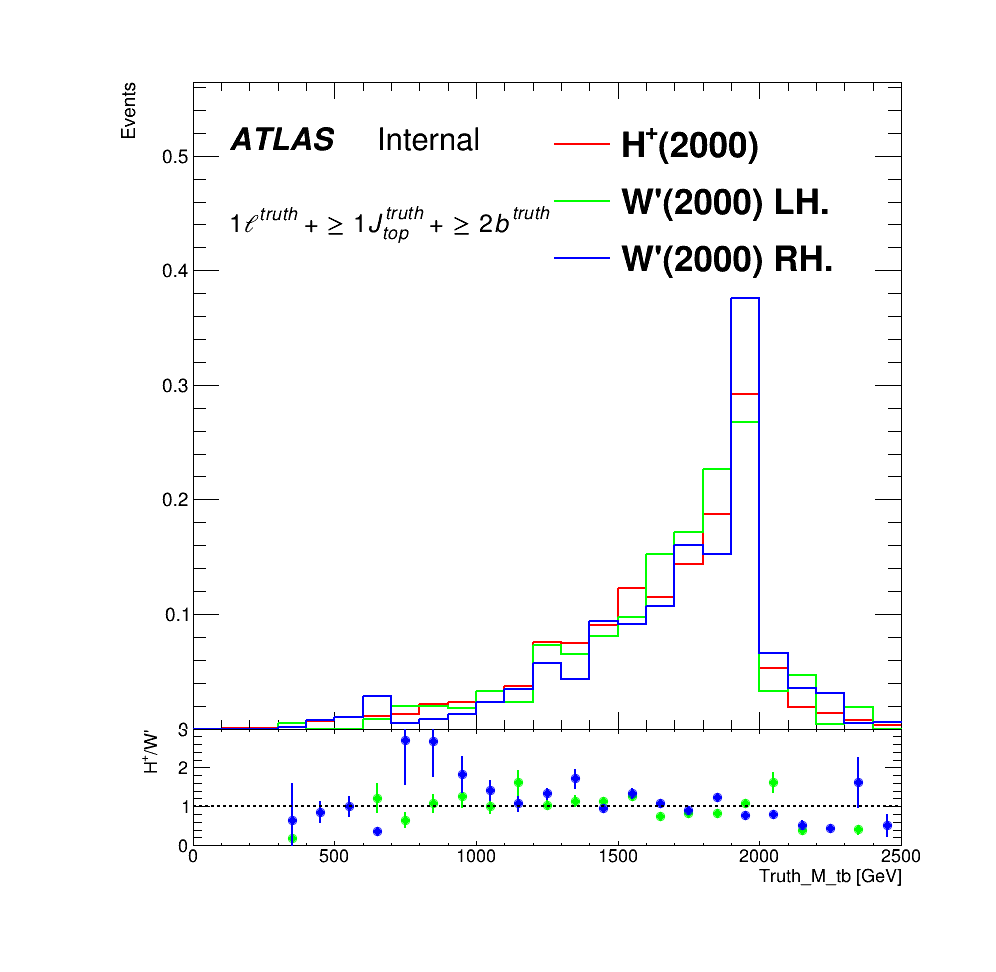
\includegraphics[width=0.25\textwidth]{images/WpMCTest/Comparison_tb_m_2000GeV.png}
    \label{fig:HpOVERWp_tb_mass_2000GeV}
  }\\
  \subfloat[Truth\_Pt\_tb] {
    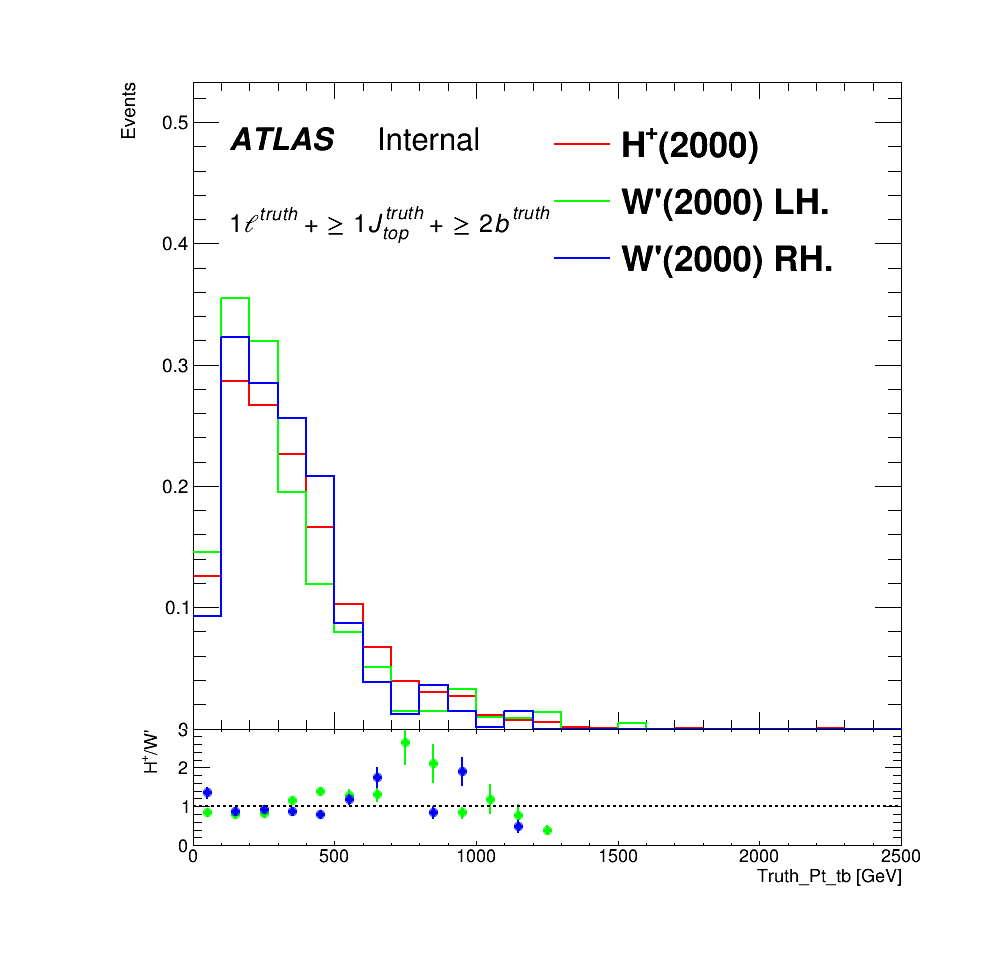
\includegraphics[width=0.25\textwidth]{images/WpMCTest/Comparison_tb_pt_2000GeV.png}
    \label{fig:HpOVERWp_tb_pt_2000GeV}
  }
  \subfloat[Truth\_PtAsymm\_tb] {
    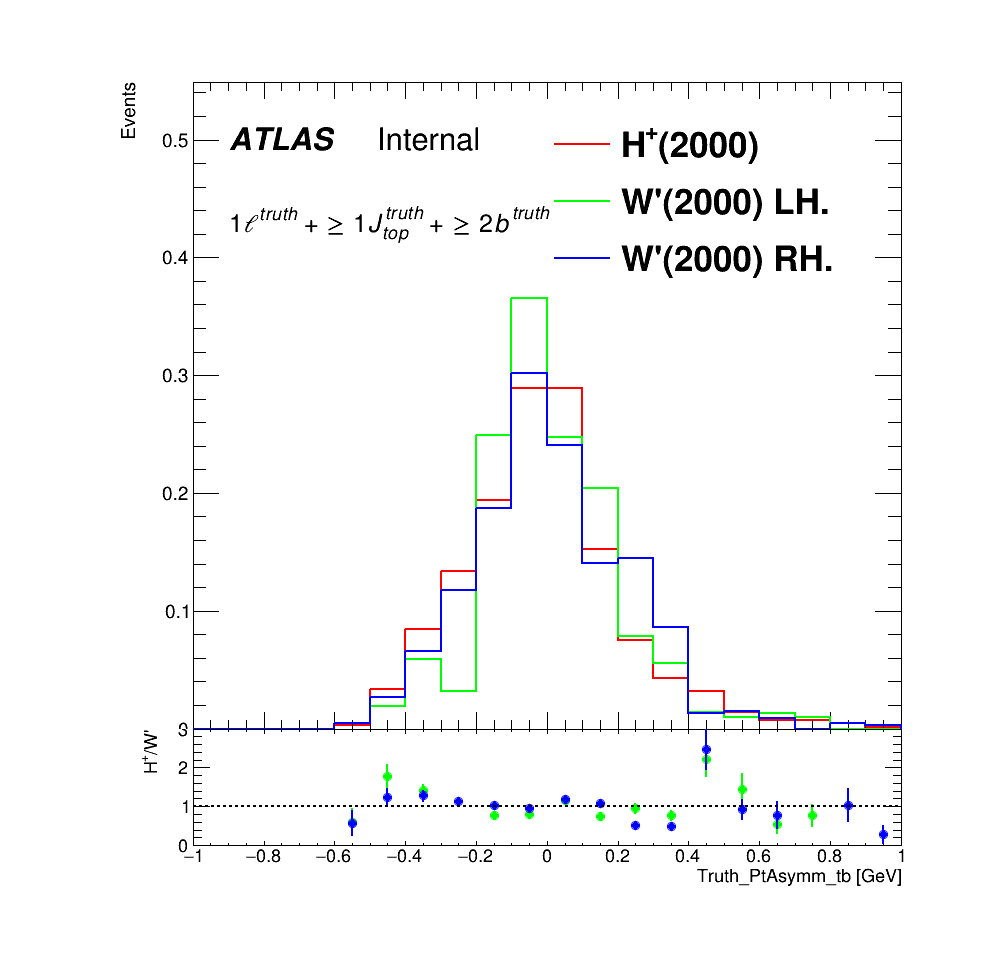
\includegraphics[width=0.25\textwidth]{images/WpMCTest/Comparison_tb_ptAsymm_2000GeV.png}
    \label{fig:HpOVERWp_tb_ptAsymm_2000GeV}
  }
  \caption{Comparison of the kinematic variables between $tbW'$ and $tbH^{+}$ in truth level on 2000 GeV mass hypothesis.}
  \label{fig:HpOVERWp_TruthLevel_2000GeV}
\end{figure}


\begin{figure}[H]
  \subfloat[Truth\_HT\_jets] {
    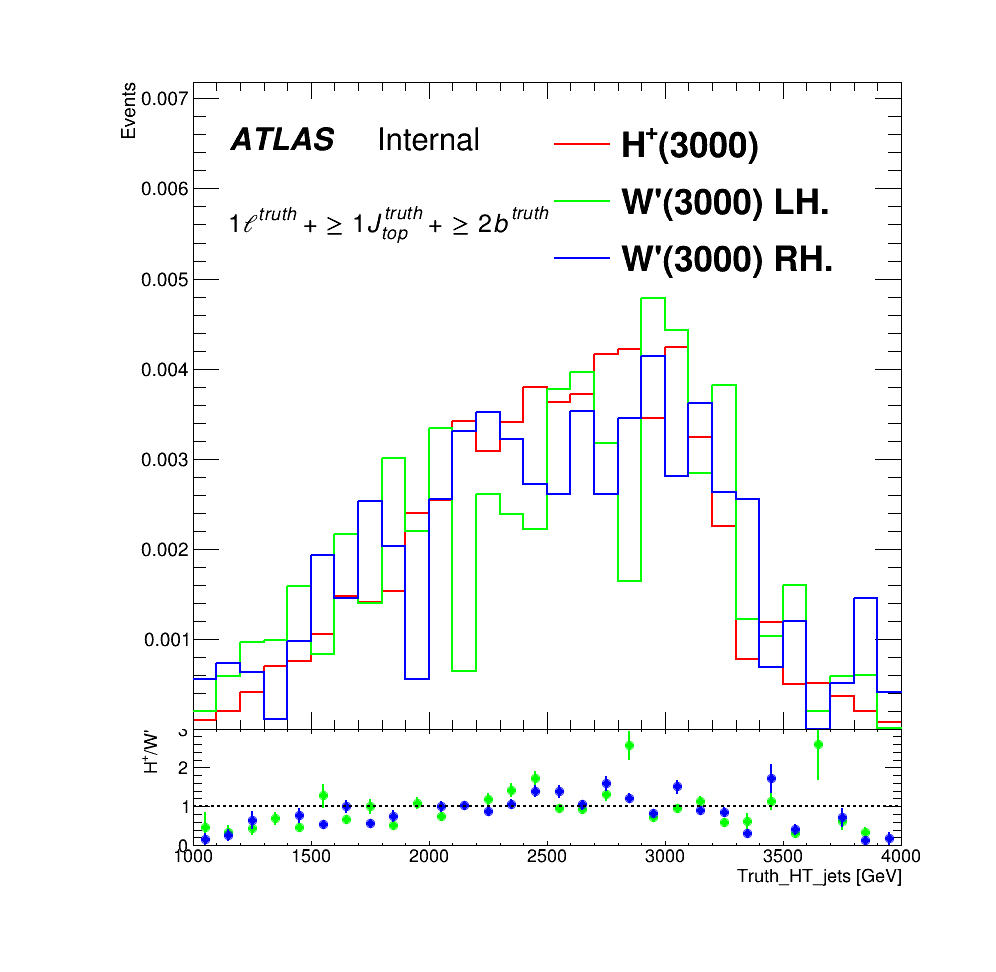
\includegraphics[width=0.25\textwidth]{images/WpMCTest/Comparison_HT_jets_3000GeV.png}
    \label{fig:HpOVERWp_HT_jets_3000GeV}
  }
  \subfloat[Truth\_LeadingJet\_pt] {
    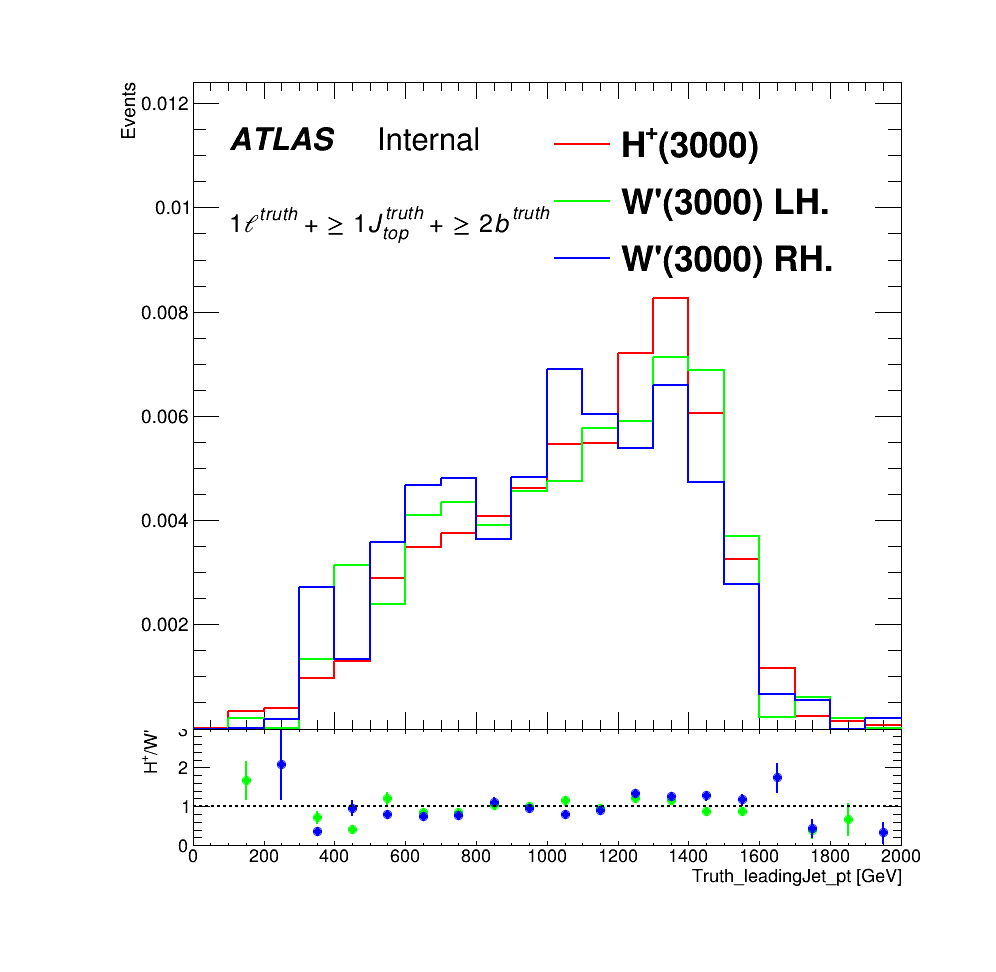
\includegraphics[width=0.25\textwidth]{images/WpMCTest/Comparison_leadingJet_pt_3000GeV.png}
    \label{fig:HpOVERWp_LeadingJet_pt_3000GeV}
  }
  \subfloat[Truth\_Centrality\_all] {
    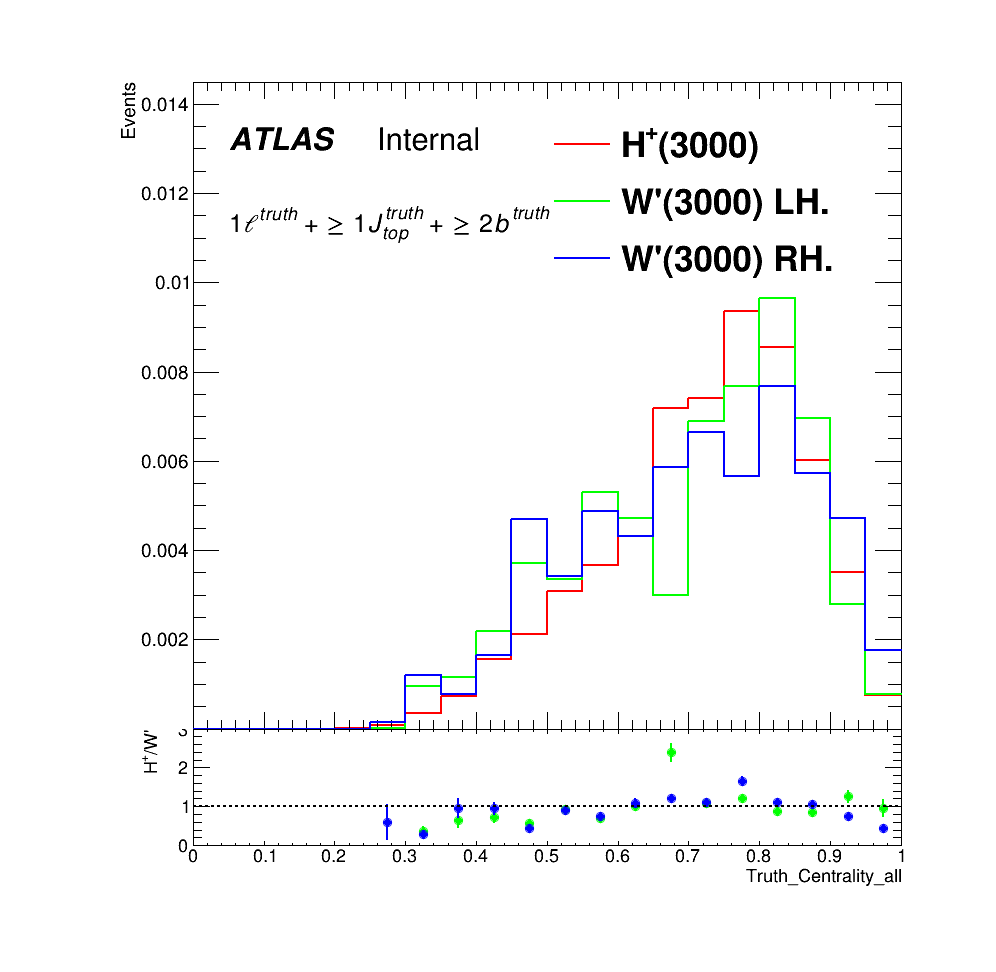
\includegraphics[width=0.25\textwidth]{images/WpMCTest/Comparison_Centrality_all_3000GeV.png}
    \label{fig:HpOVERWp_Centrality_all_3000GeV}
  }
  \subfloat[Truth\_H1\_all] {
    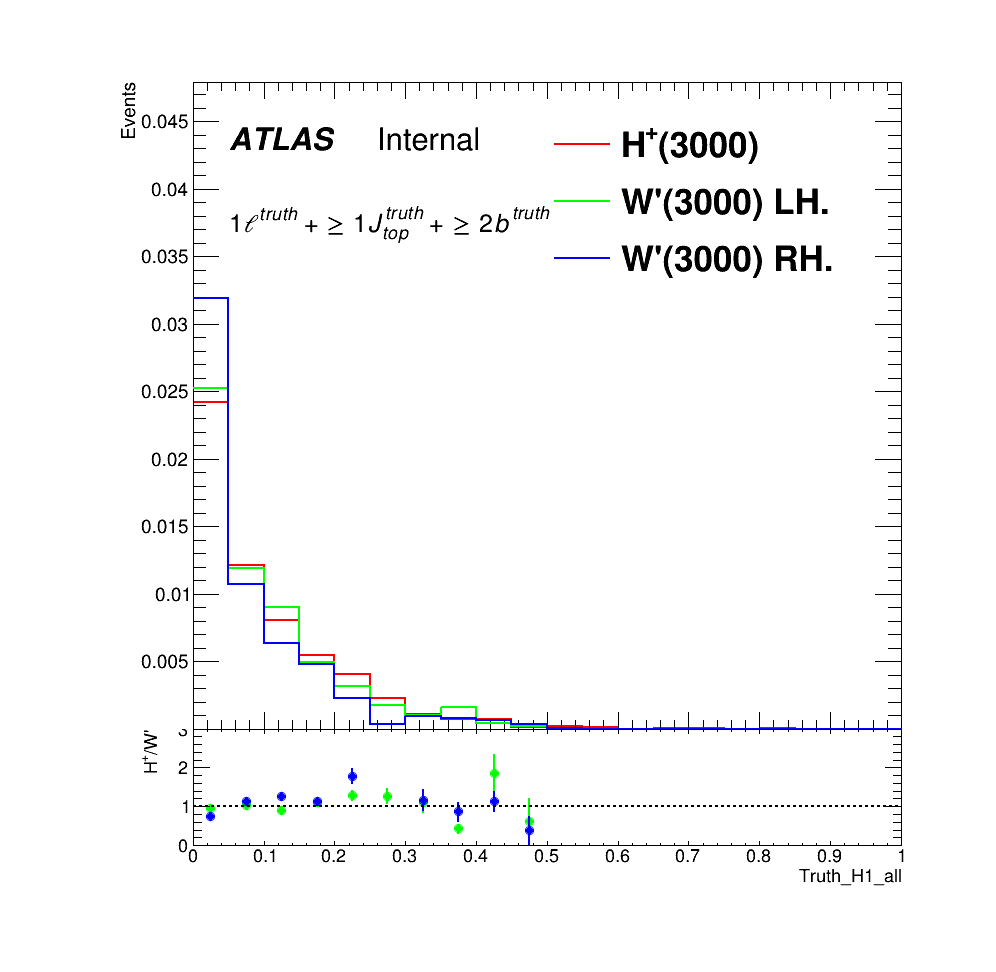
\includegraphics[width=0.25\textwidth]{images/WpMCTest/Comparison_H1_all_3000GeV.png}
    \label{fig:HpOVERWp_H1_all_3000GeV}
  }\\
  \subfloat[Truth\_Mbb\_MaxPt] {
    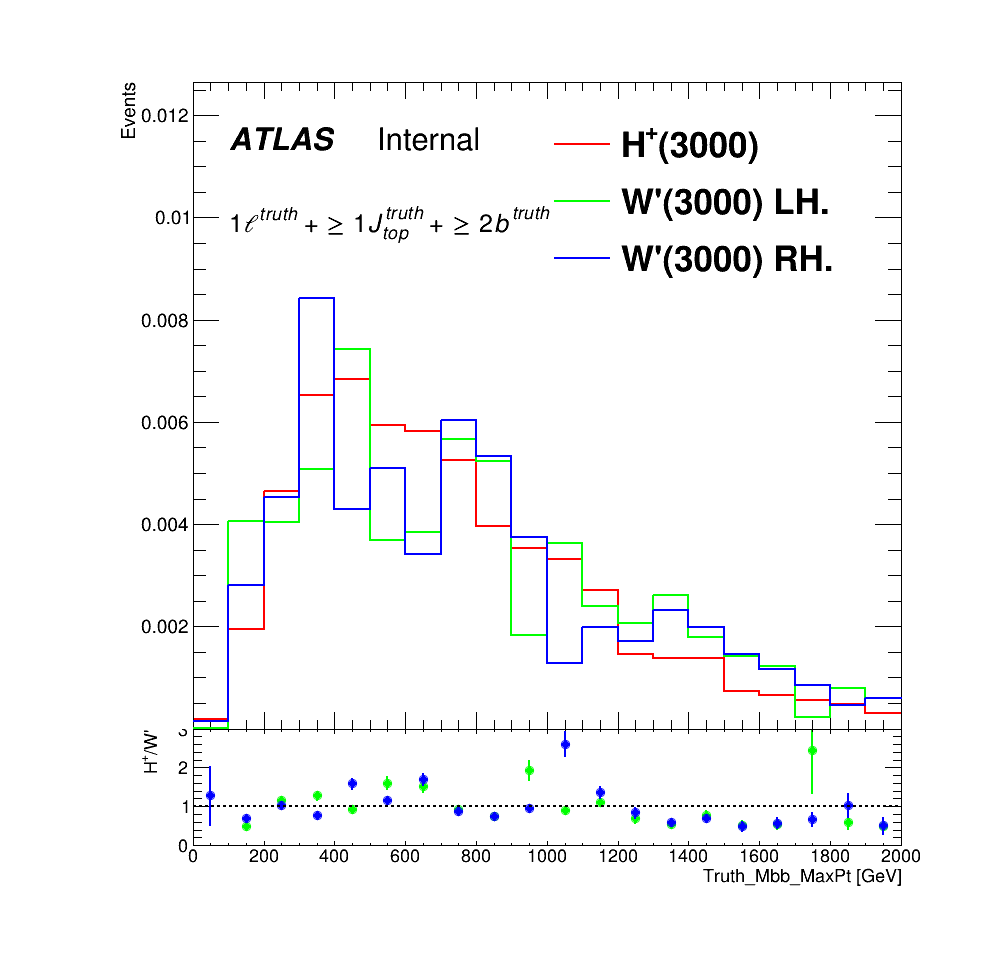
\includegraphics[width=0.25\textwidth]{images/WpMCTest/Comparison_Mbb_MaxPt_3000GeV.png}
    \label{fig:HpOVERWp_Mbb_MaxPt_3000GeV}
  }
  \subfloat[Truth\_Mjjj\_MaxPt] {
    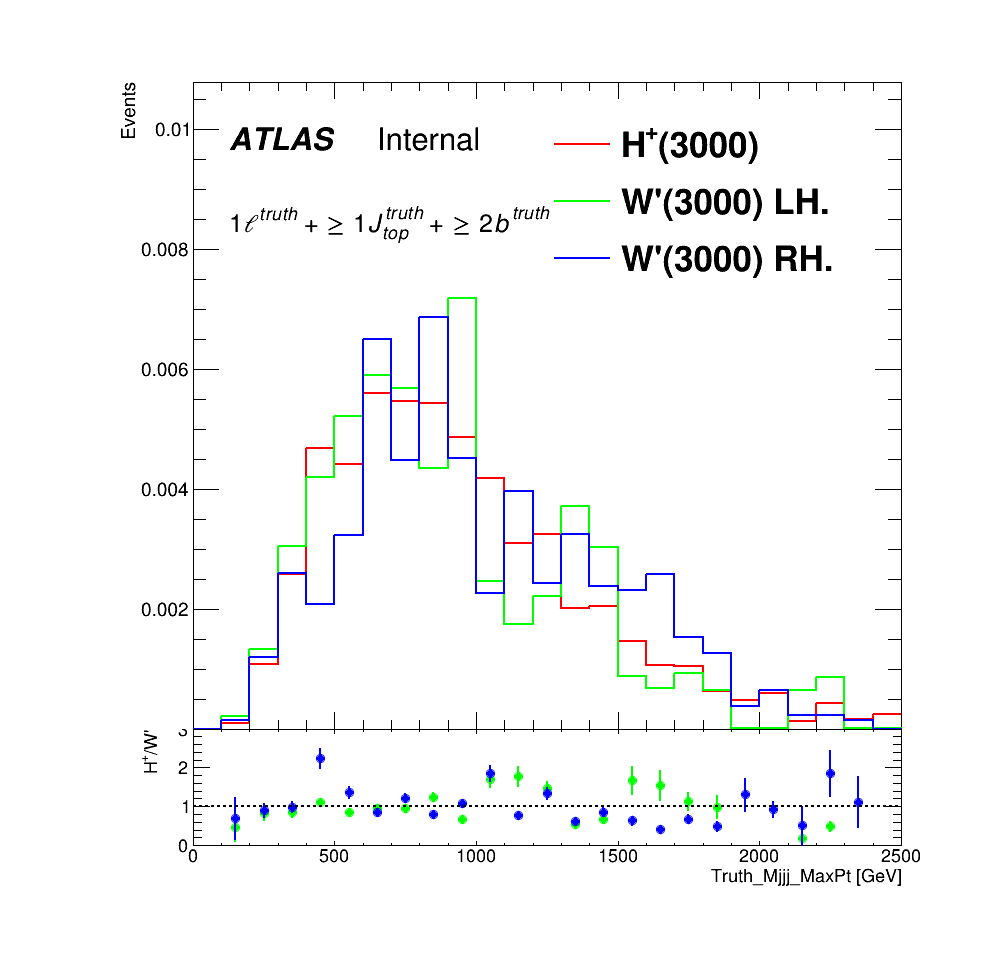
\includegraphics[width=0.25\textwidth]{images/WpMCTest/Comparison_Mjjj_MaxPt_3000GeV.png}
    \label{fig:HpOVERWp_Mjjj_MaxPt_3000GeV}
  }
  \subfloat[Truth\_Muu\_MindR] {
    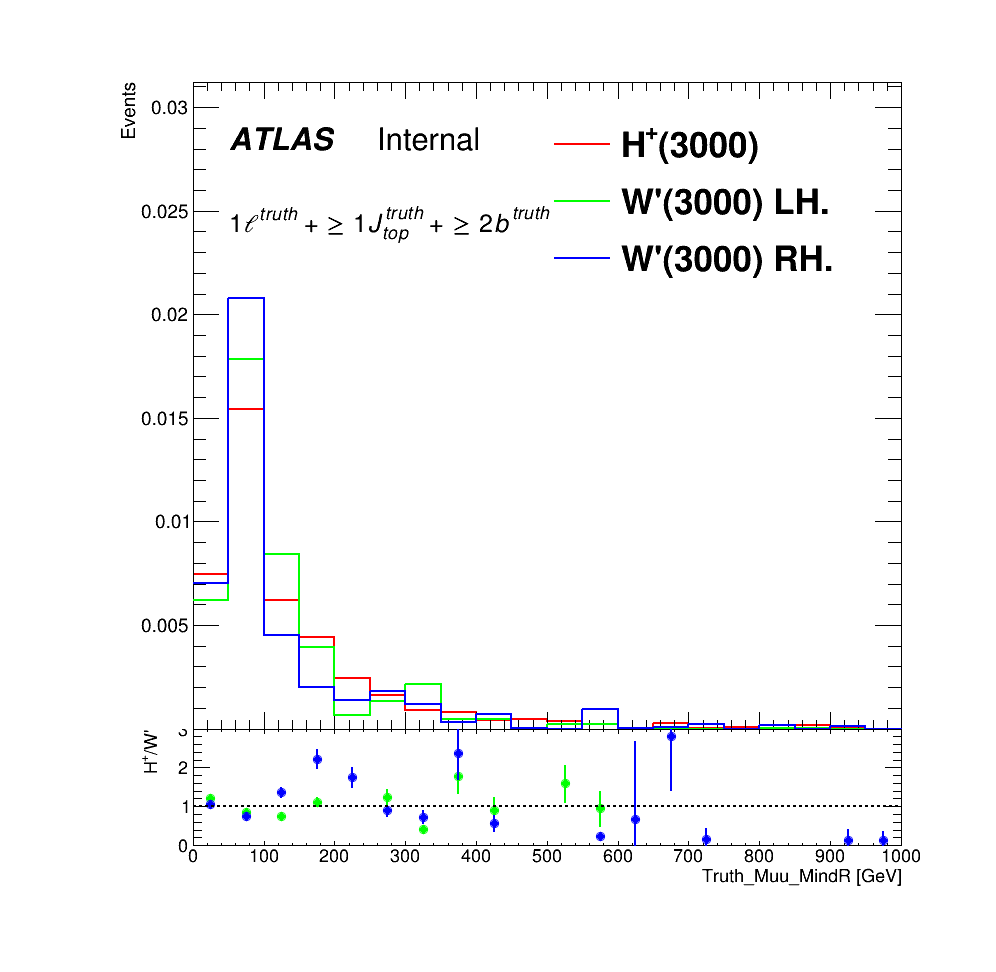
\includegraphics[width=0.25\textwidth]{images/WpMCTest/Comparison_Muu_MindR_3000GeV.png}
    \label{fig:HpOVERWp_Muu_MindR_3000GeV}
  }
  \subfloat[Truth\_dRbb\_avg] {
    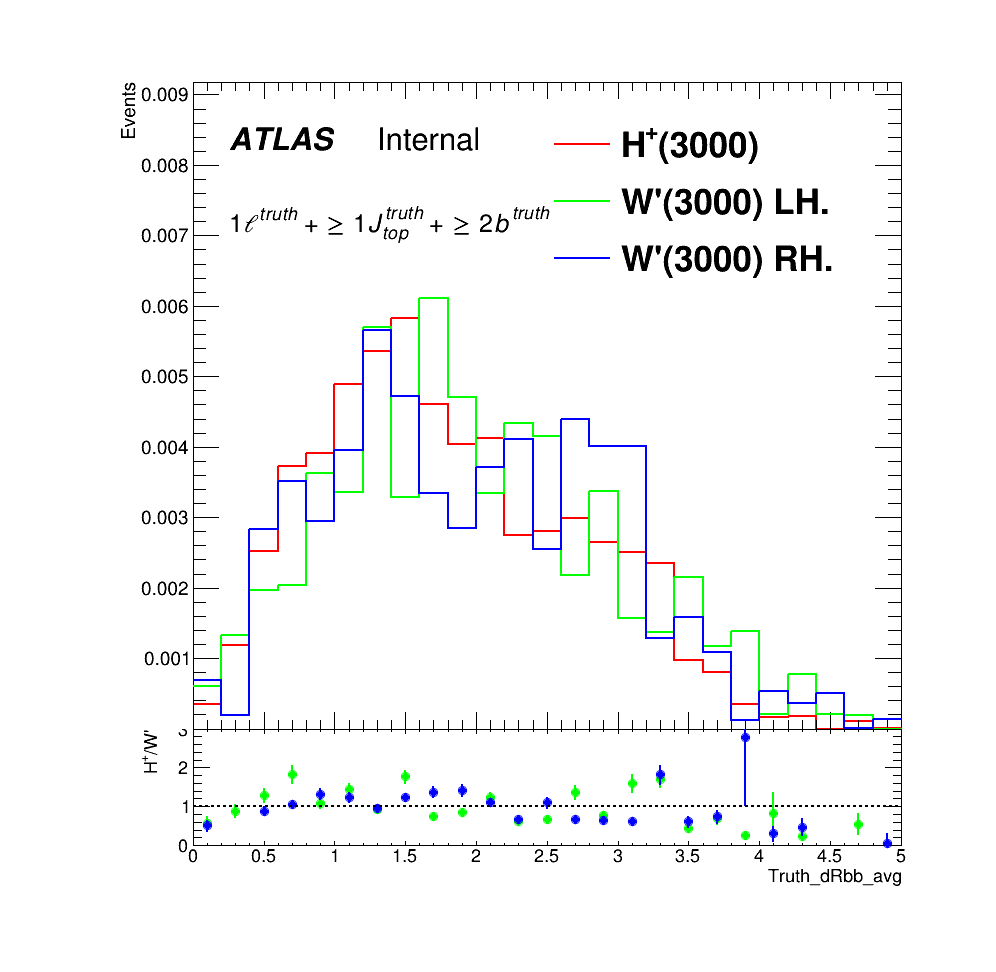
\includegraphics[width=0.25\textwidth]{images/WpMCTest/Comparison_dRbb_avg_3000GeV.png}
    \label{fig:HpOVERWp_dRbb_avg_3000GeV}
  }\\
  \subfloat[Truth\_dRlepbb\_MindR] {
    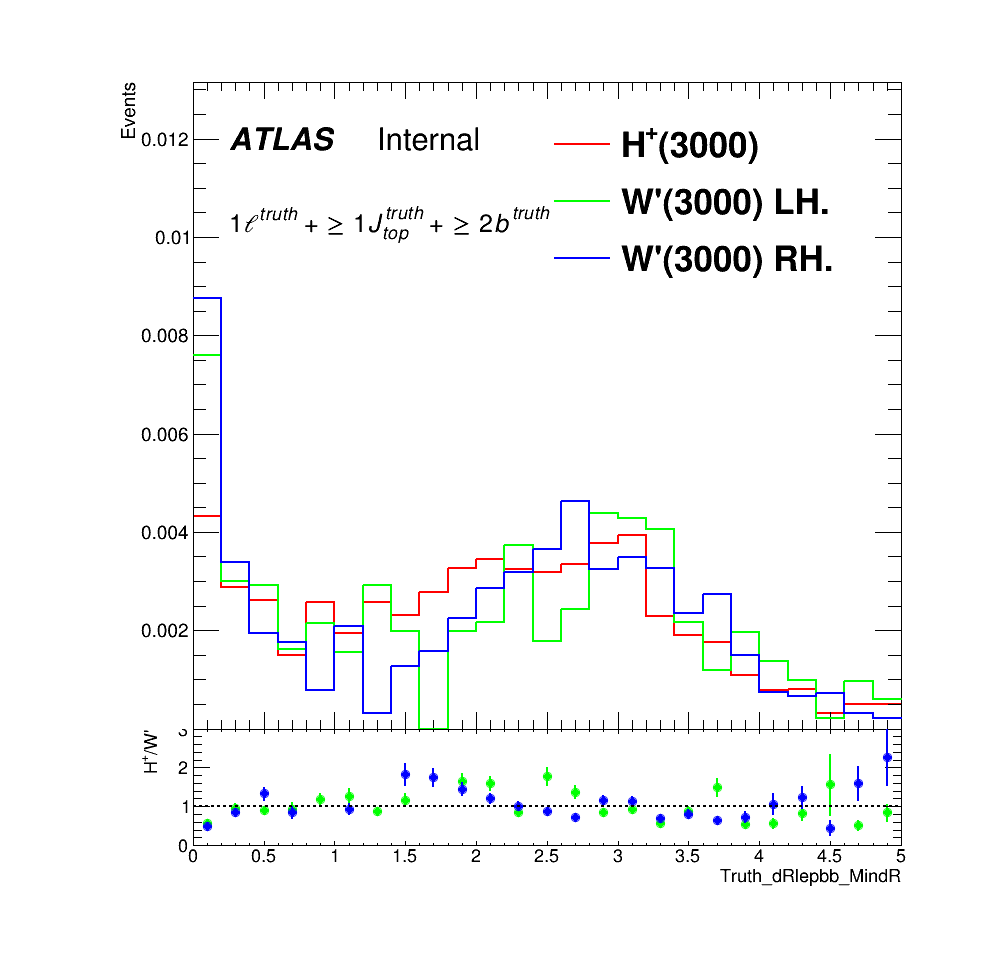
\includegraphics[width=0.25\textwidth]{images/WpMCTest/Comparison_dRlepbb_MindR_3000GeV.png}
    \label{fig:HpOVERWp_dRlepbb_MindR_3000GeV}
  }
  \subfloat[Truth\_LeadingTop\_m] {
    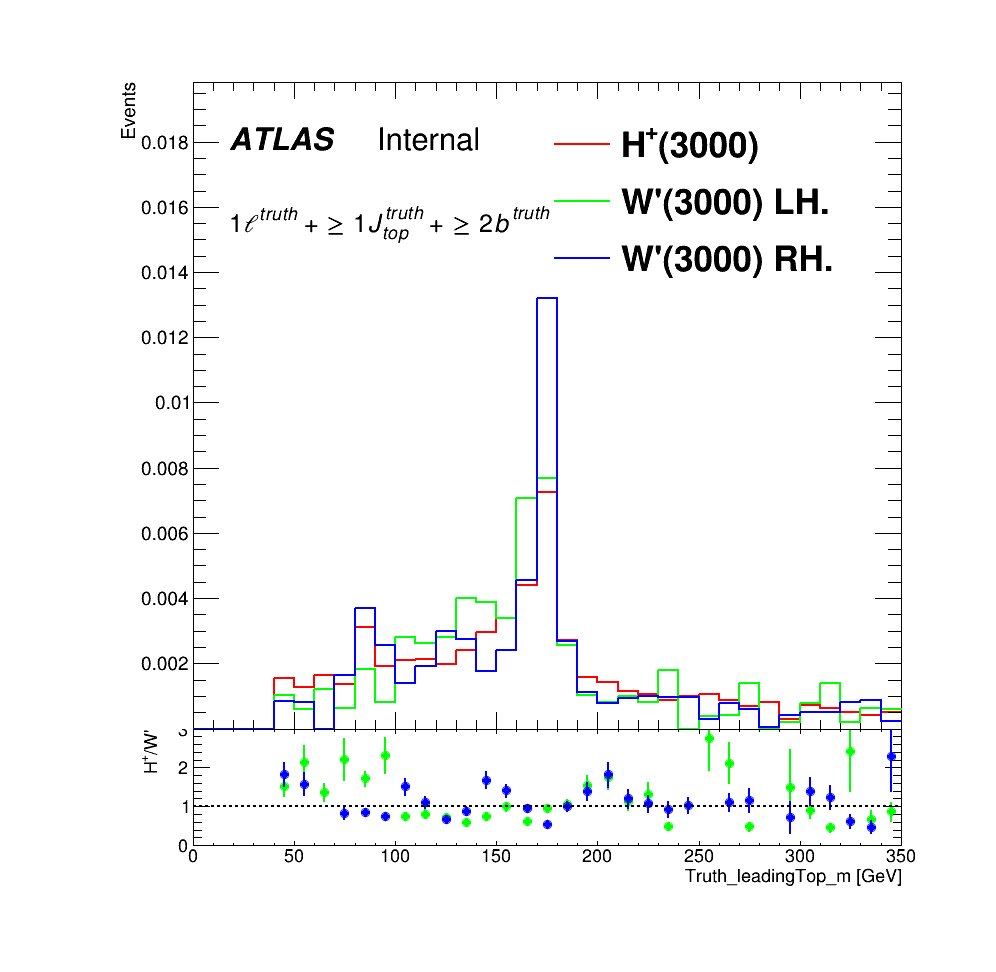
\includegraphics[width=0.25\textwidth]{images/WpMCTest/Comparison_leadingTop_m_3000GeV.png}
    \label{fig:HpOVERWp_LeadingTop_mass_3000GeV}
  }
  \subfloat[Truth\_LeadingTop\_pt] {
    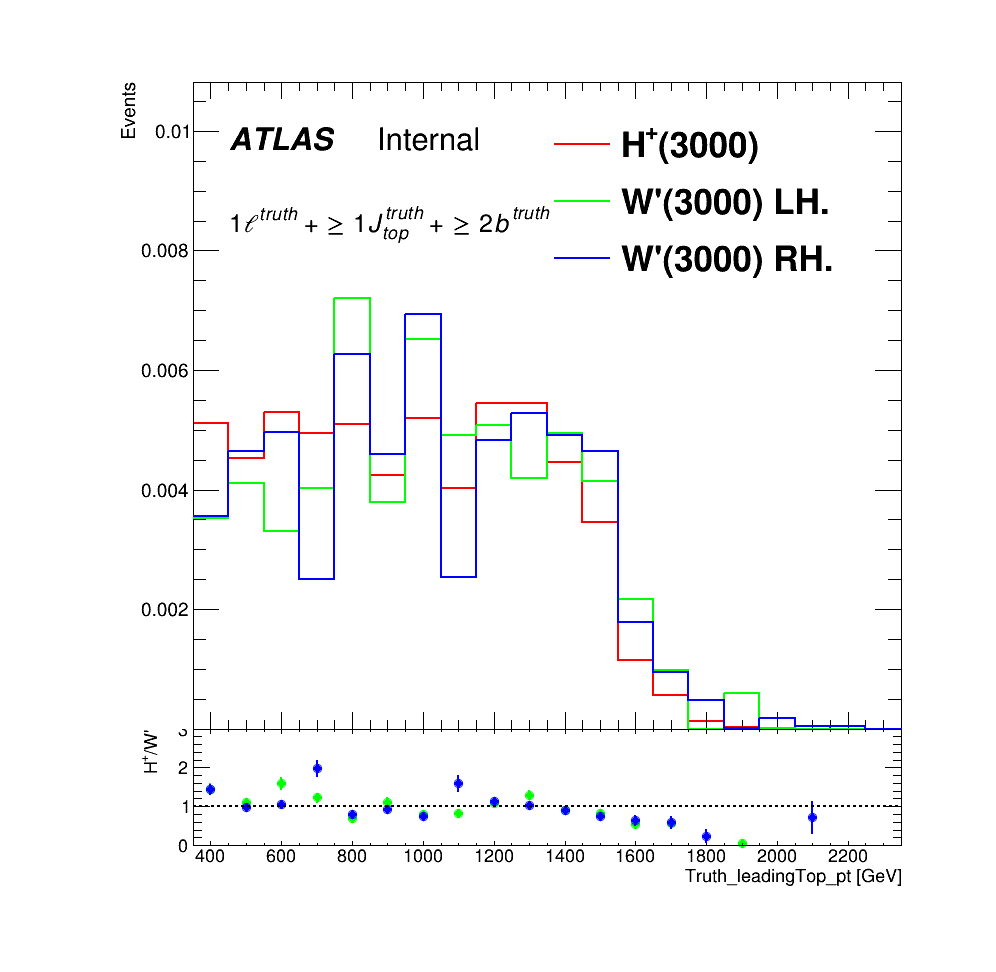
\includegraphics[width=0.25\textwidth]{images/WpMCTest/Comparison_leadingTop_pt_3000GeV.png}
    \label{fig:HpOVERWp_LeadingTop_pt_3000GeV}
  }
  \subfloat[Truth\_M\_tb] {
    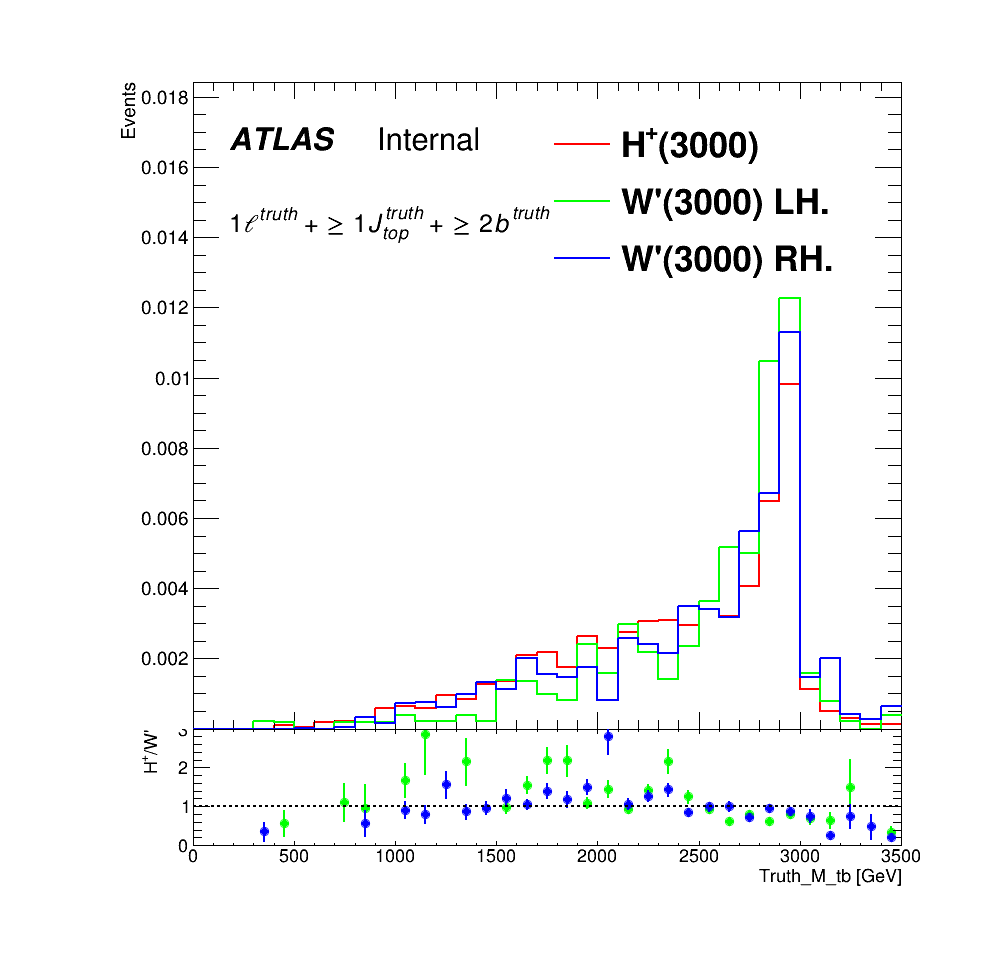
\includegraphics[width=0.25\textwidth]{images/WpMCTest/Comparison_tb_m_3000GeV.png}
    \label{fig:HpOVERWp_tb_mass_3000GeV}
  }\\
  \subfloat[Truth\_Pt\_tb] {
    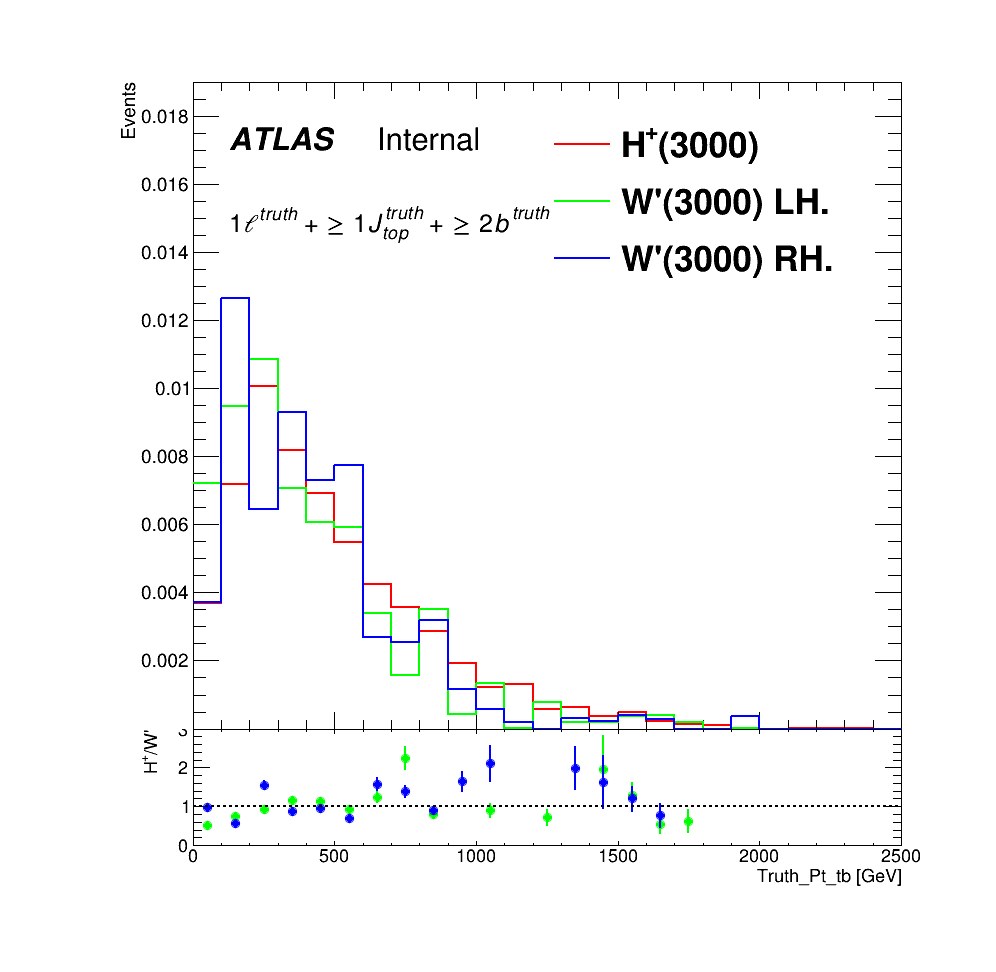
\includegraphics[width=0.25\textwidth]{images/WpMCTest/Comparison_tb_pt_3000GeV.png}
    \label{fig:HpOVERWp_tb_pt_3000GeV}
  }
  \subfloat[Truth\_PtAsymm\_tb] {
    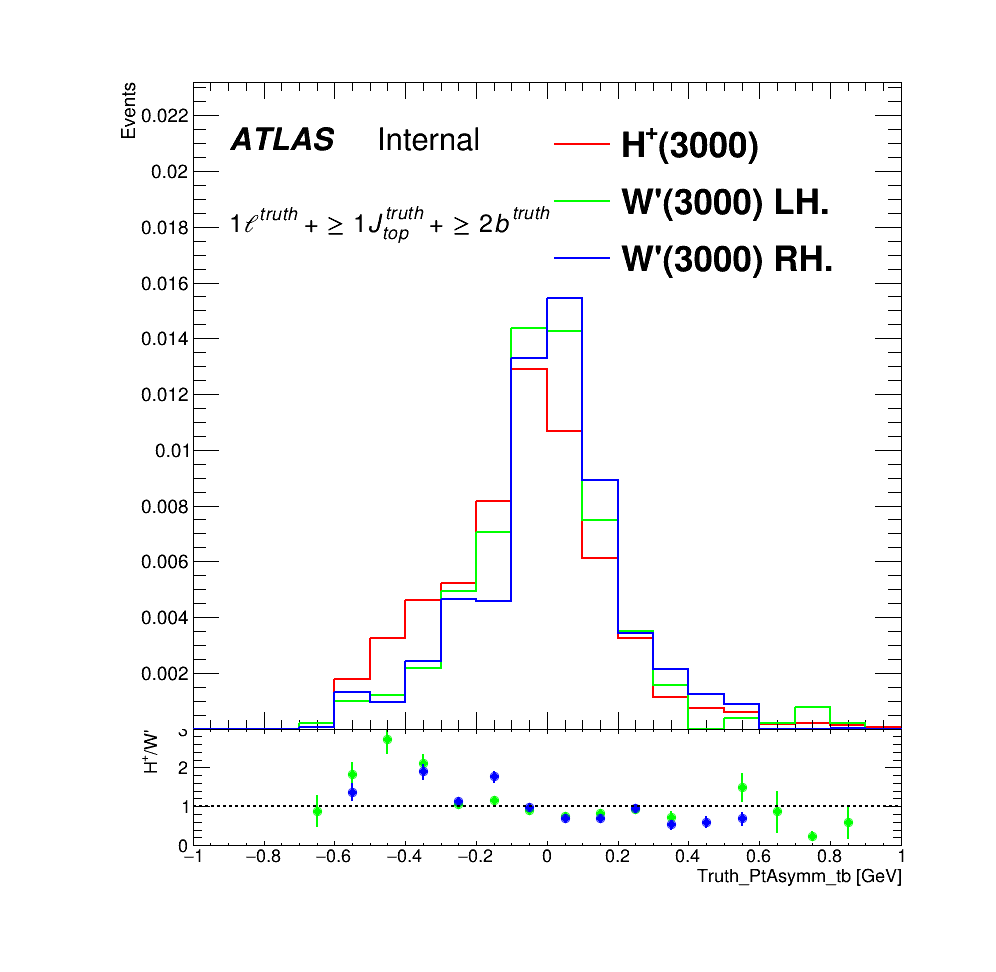
\includegraphics[width=0.25\textwidth]{images/WpMCTest/Comparison_tb_ptAsymm_3000GeV.png}
    \label{fig:HpOVERWp_tb_ptAsymm_3000GeV}
  }
  \caption{Comparison of the kinematic variables between $tbW'$ and $tbH^{+}$ in truth level on 3000 GeV mass hypothesis.}
  \label{fig:HpOVERWp_TruthLevel_3000GeV}
\end{figure}

\begin{figure}[H]
  \subfloat[Truth\_HT\_jets] {
    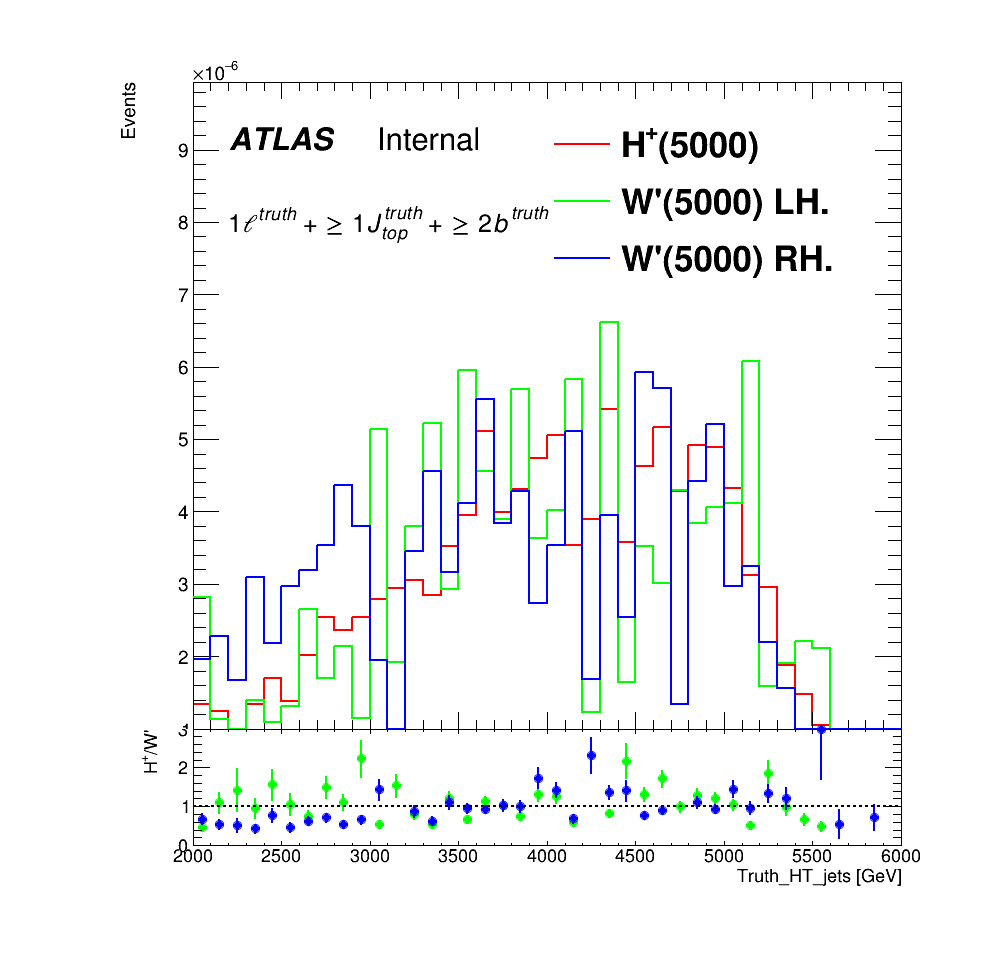
\includegraphics[width=0.25\textwidth]{images/WpMCTest/Comparison_HT_jets_5000GeV.png}
    \label{fig:HpOVERWp_HT_jets_5000GeV}
  }
  \subfloat[Truth\_LeadingJet\_pt] {
    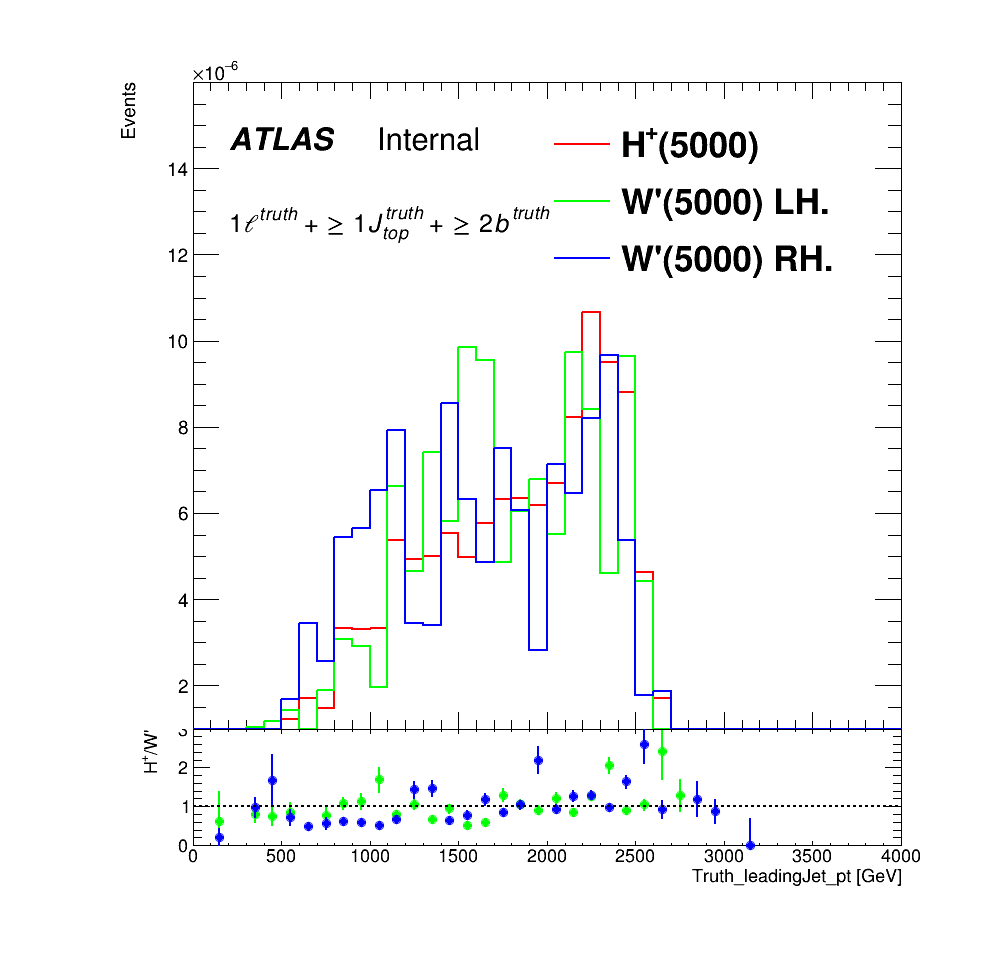
\includegraphics[width=0.25\textwidth]{images/WpMCTest/Comparison_leadingJet_pt_5000GeV.png}
    \label{fig:HpOVERWp_LeadingJet_pt_5000GeV}
  }
  \subfloat[Truth\_Centrality\_all] {
    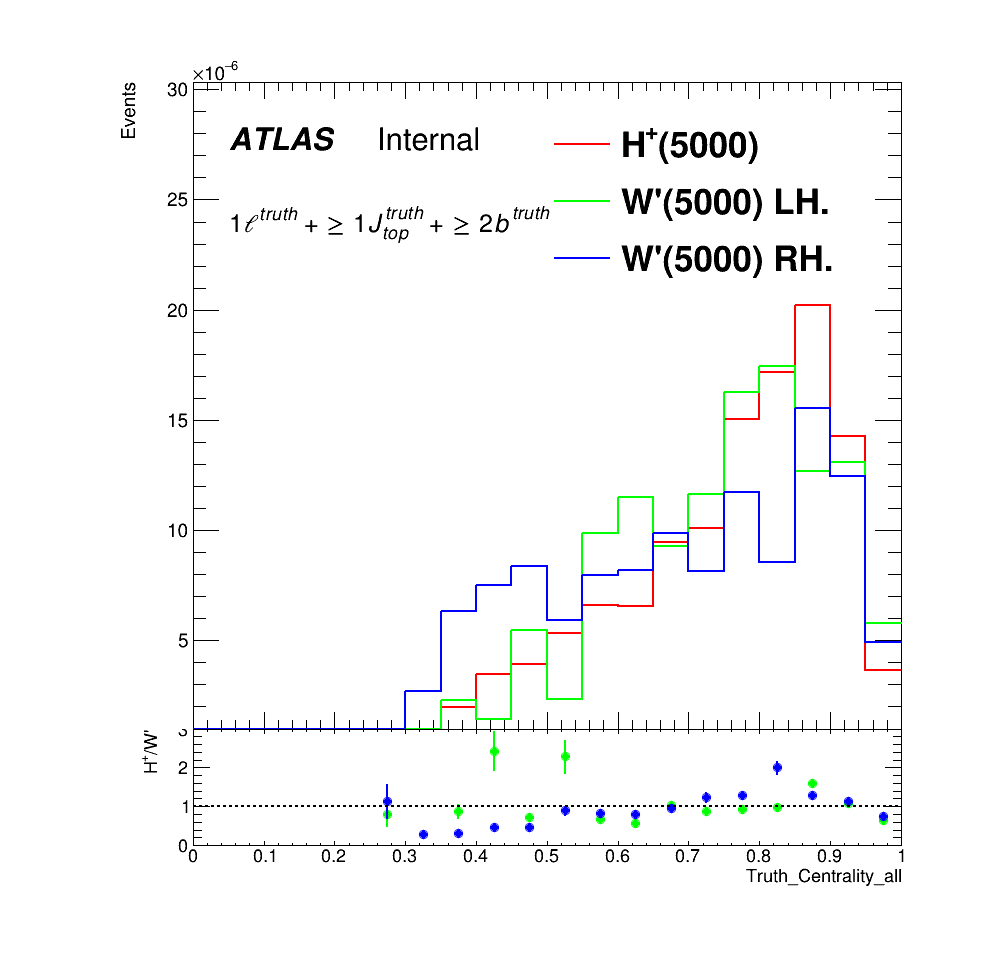
\includegraphics[width=0.25\textwidth]{images/WpMCTest/Comparison_Centrality_all_5000GeV.png}
    \label{fig:HpOVERWp_Centrality_all_5000GeV}
  }
  \subfloat[Truth\_H1\_all] {
    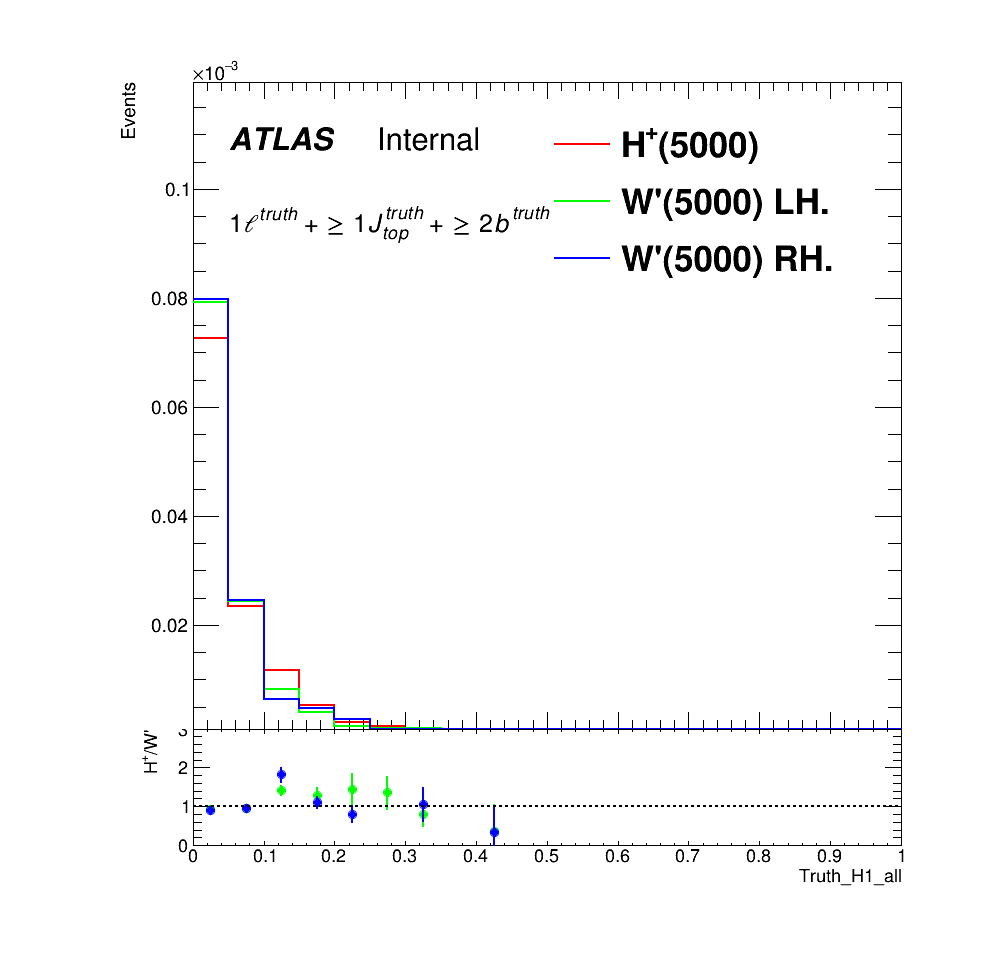
\includegraphics[width=0.25\textwidth]{images/WpMCTest/Comparison_H1_all_5000GeV.png}
    \label{fig:HpOVERWp_H1_all_5000GeV}
  }\\
  \subfloat[Truth\_Mbb\_MaxPt] {
    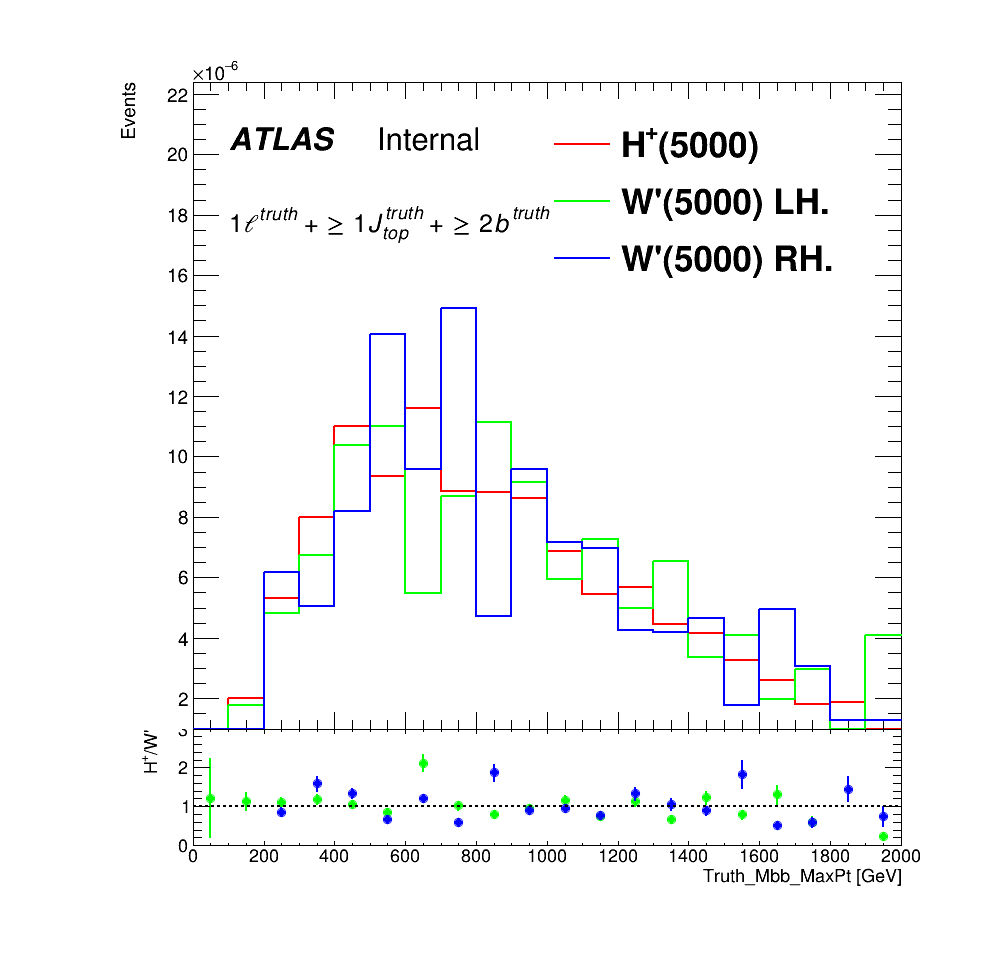
\includegraphics[width=0.25\textwidth]{images/WpMCTest/Comparison_Mbb_MaxPt_5000GeV.png}
    \label{fig:HpOVERWp_Mbb_MaxPt_5000GeV}
  }
  \subfloat[Truth\_Mjjj\_MaxPt] {
    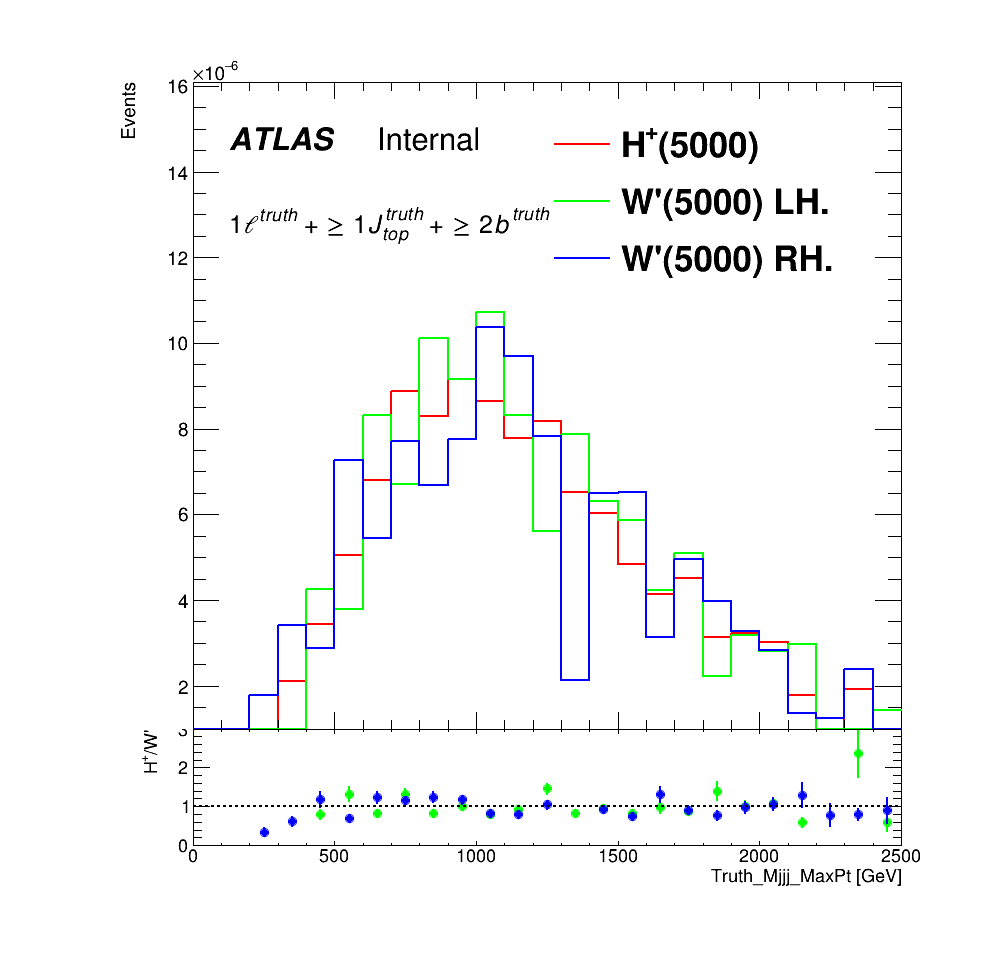
\includegraphics[width=0.25\textwidth]{images/WpMCTest/Comparison_Mjjj_MaxPt_5000GeV.png}
    \label{fig:HpOVERWp_Mjjj_MaxPt_5000GeV}
  }
  \subfloat[Truth\_Muu\_MindR] {
    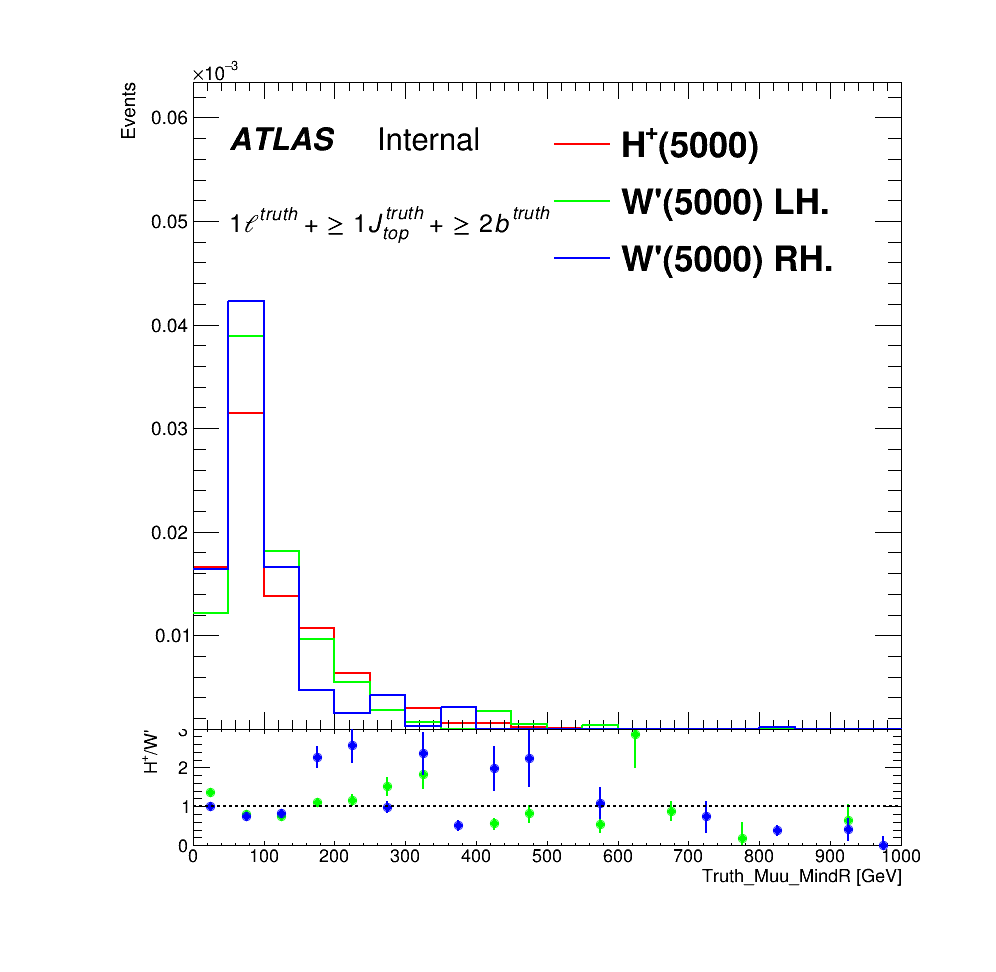
\includegraphics[width=0.25\textwidth]{images/WpMCTest/Comparison_Muu_MindR_5000GeV.png}
    \label{fig:HpOVERWp_Muu_MindR_5000GeV}
  }
  \subfloat[Truth\_dRbb\_avg] {
    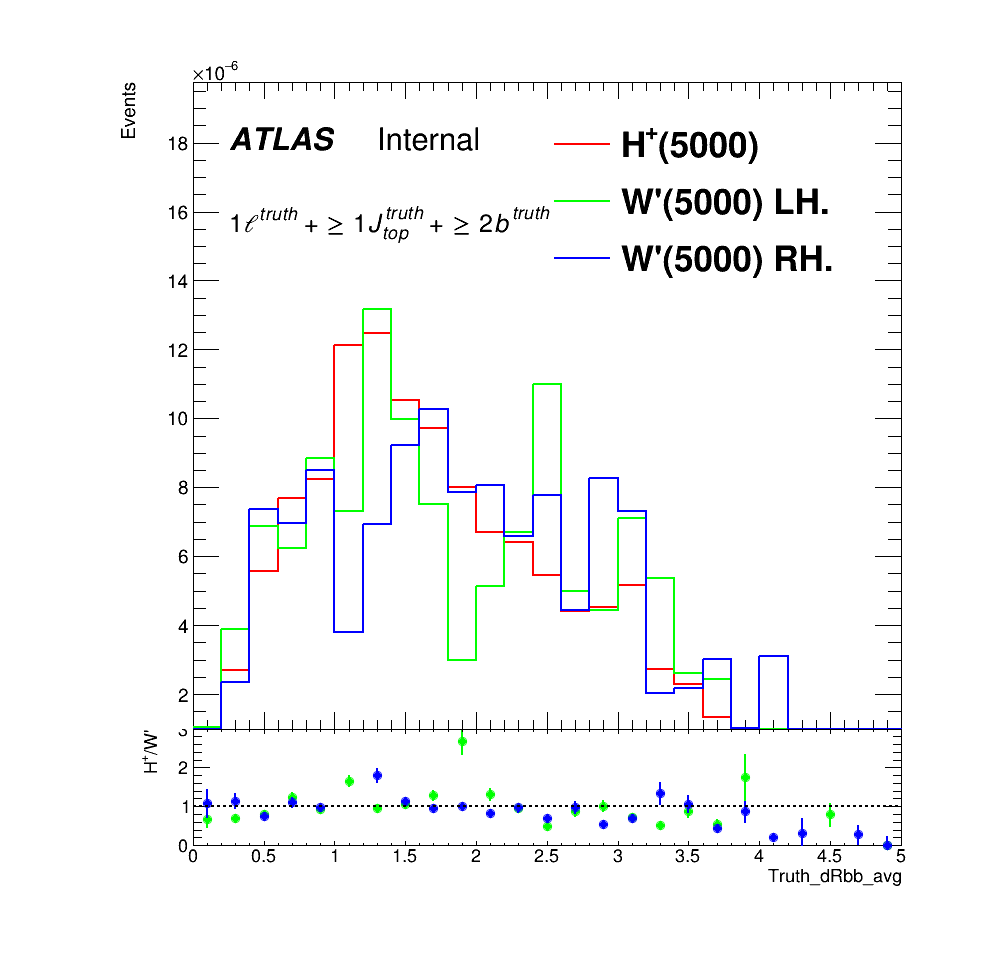
\includegraphics[width=0.25\textwidth]{images/WpMCTest/Comparison_dRbb_avg_5000GeV.png}
    \label{fig:HpOVERWp_dRbb_avg_5000GeV}
  }\\
  \subfloat[Truth\_dRlepbb\_MindR] {
    \includegraphics[width=0.25\textwidth]{images/WpMCTest/Comparison_dRlepbb_MindR_5000GeV.png}
    \label{fig:HpOVERWp_dRlepbb_MindR_5000GeV}
  }
  \subfloat[Truth\_LeadingTop\_m] {
    \includegraphics[width=0.25\textwidth]{images/WpMCTest/Comparison_leadingTop_m_5000GeV.png}
    \label{fig:HpOVERWp_LeadingTop_mass_5000GeV}
  }
  \subfloat[Truth\_LeadingTop\_pt] {
    \includegraphics[width=0.25\textwidth]{images/WpMCTest/Comparison_leadingTop_pt_5000GeV.png}
    \label{fig:HpOVERWp_LeadingTop_pt_5000GeV}
  }
  \subfloat[Truth\_M\_tb] {
    \includegraphics[width=0.25\textwidth]{images/WpMCTest/Comparison_tb_m_5000GeV.png}
    \label{fig:HpOVERWp_tb_mass_5000GeV}
  }\\
  \subfloat[Truth\_Pt\_tb] {
    \includegraphics[width=0.25\textwidth]{images/WpMCTest/Comparison_tb_pt_5000GeV.png}
    \label{fig:HpOVERWp_tb_pt_5000GeV}
  }
  \subfloat[Truth\_PtAsymm\_tb] {
    \includegraphics[width=0.25\textwidth]{images/WpMCTest/Comparison_tb_ptAsymm_5000GeV.png}
    \label{fig:HpOVERWp_tb_ptAsymm_5000GeV}
  }
  \caption{Comparison of the kinematic variables between $tbW'$ and $tbH^{+}$ in truth level on 5000 GeV mass hypothesis.}
  \label{fig:HpOVERWp_TruthLevel_5000GeV}
\end{figure}
